%!TEX root = root.tex

\chapter{A Law of Large Graphs}
\label{chap:llg}

Estimation of the mean of a population based on samples is at the core of statistics.
The sample mean, motivated by the law of large numbers and the central limit theorem, has its place as one of the most important statistics for this task.
In modern settings, we take averages almost everywhere, from data in Euclidean space to more complex objects like images, shapes, and documents.
In this chapter we consider the challenges of estimating a population mean based on a sample of graphs, for example the human brains as represented by their structural connectomes. 

The mean of a population of graphs is a high dimensional object, consisting of $O(n^2)$ parameters for graphs with $n$ vertices.
When the number of samples $m$ is much smaller than $n^2$, or even $n$, estimating such high dimensional estimands using naive unbiased methods often leads to inaccurate estimates with very high variance.
Furthermore, using these estimates for subsequent inference tasks such as testing can lead to low power and accuracy.
By exploiting a bias-variance trade-off, it is often fruitful to develop estimators which have some bias but greatly reduced variance.
When these estimators are biased towards low-dimensional structures which well approximate the full dimensional population mean, major improvements can be realized \citep{trunk1979problem}.

In a striking result, \citet{stein1956inadmissibility} and \citet{james1961estimation} showed that even the arithmetic mean can be dominated by another procedure.
In particular, James and Stein showed that the sample mean for a multivariate normal distribution with at least three dimensions has strictly higher risk than a procedure that introduces shrinkage, and can be strictly improved by carefully biasing the  estimate towards any given fixed point. 
Twenty-seven years later, \citet{gutmann1982stein} proved that this phenomenon cannot occur when the sample spaces are finite, as is the case for graphs.
However, while there must be some cases where the sample mean is preferred, this does not mean that other estimators should not be considered.
In many situations where other structural information is hypothesized, other estimators may be preferable.

In complex data settings such as shape data, language data, or graph data, we also must take care in how we define the mean.
For a population, we define the mean graph as the weighted adjacency matrix with weights given by the proportion of times the corresponding edge appears in the population. 
This definition naturally extends the definition of the mean for standard Euclidean data.
As with real valued data, one may want to define the mean of a population of graphs to be a graph.
This is captured in the notion of the median graph \citep{jiang2001median}, however, this may be too restrictive for populations of graphs where there is high variation in which edges appear. 
As we will describe below, our definition of the mean graph is the expectation of the adjacency matrix.

This population mean is becoming an important object for statistical inference.
For example, \citet{ginestet2014hypothesis} proposed a way to test if there is a difference between the distributions for two groups of networks.  
While hypothesis testing is the end goal of their work, estimation is a key intermediate step which may be improved by accounting for underlying structure in the mean matrix. 
Thus, improving the estimation procedures for the mean graph is not only important by itself, but also can be applied to help improve other statistical inference procedures.

To better illustrate the idea, we take the CoRR brain graphs with Desikan atlases as an example. The dataset contains 454 brain scans with 70 vertices. Each vertex represents a region defined by the Desikan atlases, while an edge exists between two vertices if there is at least one white-matter tract connecting the corresponding regions of the brain. More details about this dataset are given in Section~\ref{section:data}. By observing $m$ graphs sampled from the 454 graphs, our goal is to estimate the mean graph of the population $P$, defined as the entry-wise mean of all the 454 graphs. We plot the population mean graph $P$ on the left panel in Figure~\ref{fig:Matrix_desikan_m5}.


\begin{figure}[!tbp]
\centering
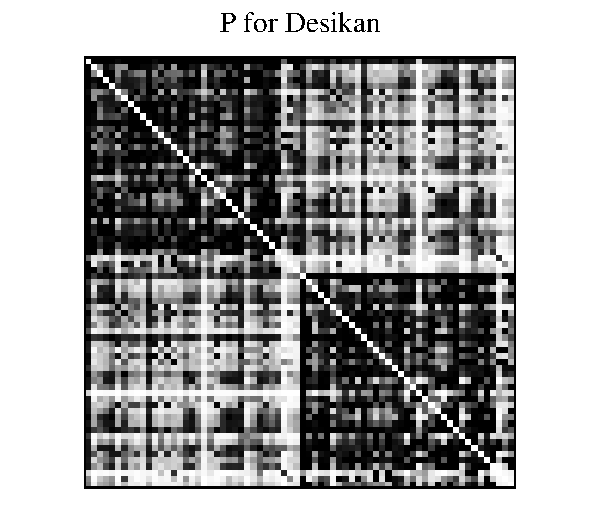
\includegraphics[height=.2\textheight]{./Figures/P_desikan.pdf} \hspace{-35pt}
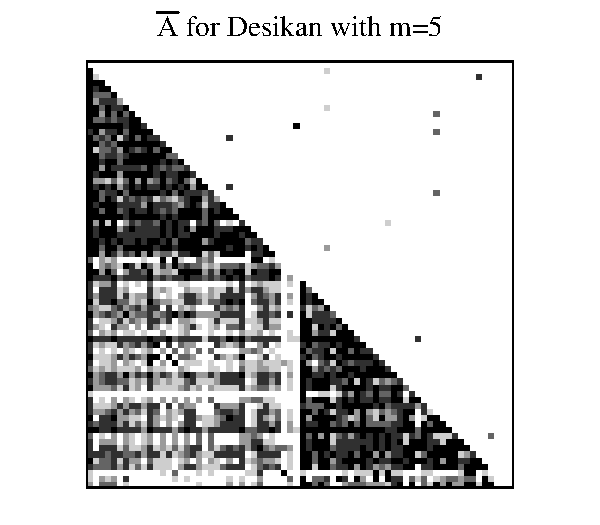
\includegraphics[height=.201\textheight]{./Figures/Abar_desikan_m5.pdf} \hspace{-35pt}
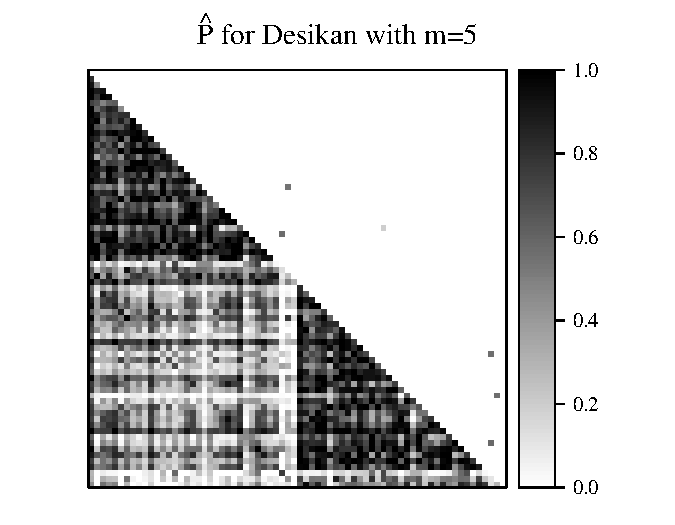
\includegraphics[height=.205\textheight]{./Figures/Phat_desikan_m5.pdf}
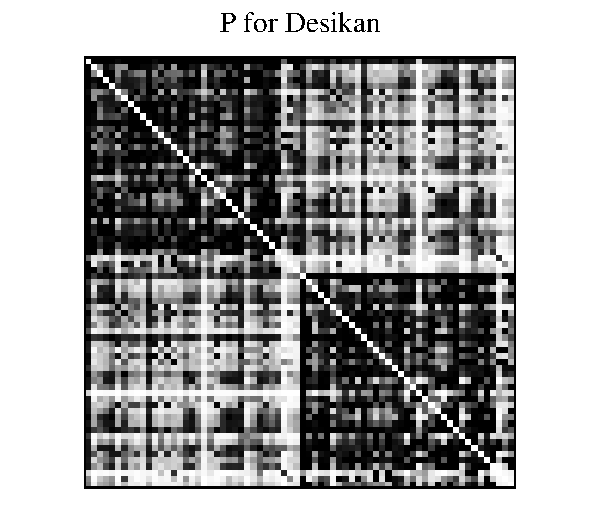
\includegraphics[height=.2\textheight]{./Figures/P_desikan.pdf} \hspace{-35pt}
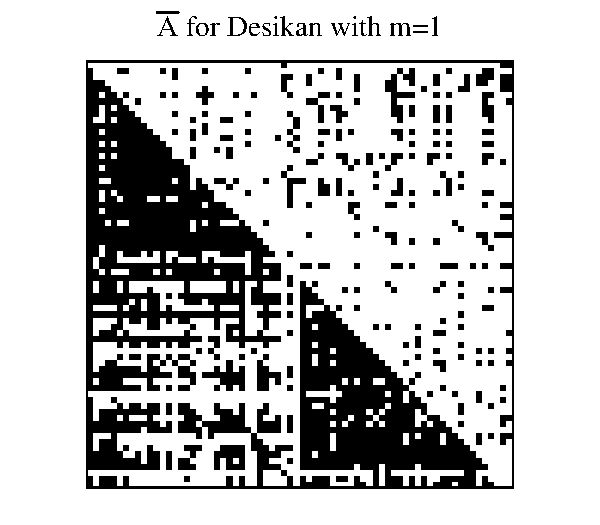
\includegraphics[height=.201\textheight]{./Figures/Abar_desikan_m1.pdf} \hspace{-35pt}
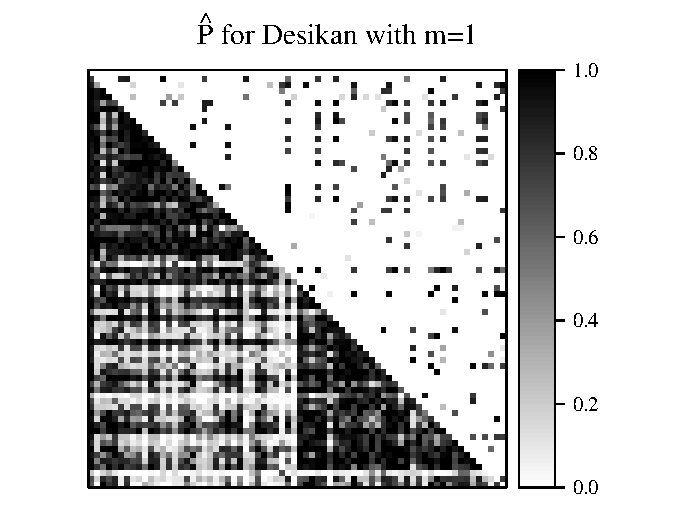
\includegraphics[height=.205\textheight]{./Figures/Phat_desikan_m1.pdf}
\caption[Heat maps of the population mean, the sample mean, and the low-rank estimator]{Heat maps of the population mean $P$, the sample mean $\bar{A}$, and the estimator $\hat{P}$ based on sample sizes $m = 1$ and $m = 5$.
The three heat maps in the upper level indicate the population mean for the $454$ graphs (left), sample mean for the 5 sampled graphs (center), and $\hat{P}$ for the same 5 sampled graphs with dimension $d=11$ selected using the Zhu and Ghodsi method (right). Details about how to construct $\hat{P}$ are discussed in Section~\ref{sec:LLG_phat}.
Darker pixels indicate a higher probability of an edge between the given vertices.
By calculating the mean squared error based on this sample, we can see that $\hat{P}$ (with mean squared error equals $0.015$) outperforms $\bar{A}$ (with mean squared error equals $0.016$), with a 3\% relative improvement.
In order to see where the improvements are clearly, in the upper triangular of the heat maps for $\bar{A}$ and $\hat{P}$, we highlight the edges (18 edges highlighted for $\bar{A}$ and 6 for $\hat{P}$) which have absolute estimation error larger than $0.4$.
In the lower level, we plot three heat maps in the similar way based on sample size $m = 1$. For this specific sampled graph, $\hat{P}$ is calculated with dimension $d = 12$. A clearly smoothing effect can be seen in the heat map of $\hat{P}$ (with mean squared error equals $0.049$), which leads to a 53\% relative improvement compared to $\bar{A}$ (with mean squared error equals $0.104$). Similarly, we use the same absolute estimation error threshold $0.4$ and highlight 504 edges for $\bar{A}$ and 234 edges for $\hat{P}$.}
\label{fig:Matrix_desikan_m5}
\end{figure}



The element-wise sample mean is a reasonable estimator if we consider the general independent edge model (IEM) \citep{bollobas2007phase} introduced in Section~\ref{sec:IEM} without taking any additional structure into account. 
However, with only a small sample size, such as when the sample size is much less than the number of vertices, it does not perform very well.
Now take a sample of size $m=5$ in the CoRR dataset example with Desikan atlases mentioned above, then we calculate the entry-wise sample mean $\bar{A}$ and plot it in the top middle panel of Figure~\ref{fig:Matrix_desikan_m5}. Darker pixels indicate a higher probability of an edge between the given vertices.
We can see $\bar{A}$ gives a fair estimate of $P$. However, there are still an amount of edges being estimated very inaccurately. In order to see these inaccurate estimates clearly, in the upper triangular of the heat maps for $\bar{A}$, we highlight the 18 edges which have absolute estimation error larger than $0.4$ based on the same color scale.
When the sample size is small, the performance of $\bar{A}$ degrades due to its high variances. Such phenomenon is most obvious when we decrease the sample size from $m = 5$ to $m = 1$.
In the bottome middle panel of Figure~\ref{fig:Matrix_desikan_m5}, we plot the heat map of $\bar{A}$ based on sample size $m = 1$. Since there is only one observed graph, $\bar{A}$ is binary and thus very bumpy. Similarly, we use the same absolute estimation error threshold $0.4$ and highlight 504 edges in the upper triangular.
Intuitively, an estimator incorporating structure in the distribution of graphs, assuming the estimator is computationally tractable, is preferable to the entry-wise sample mean. 
In general, we do not have any knowledge about this structure so it can be hard to take advantage of in practice.



One of the most important structures in graphs is the community structure in which vertices are clustered into groups that share similar connectivity structure. The stochastic blockmodel (SBM) \citep{holland1983stochastic} introduced in Section~\ref{sec:SBM} is one model that captures this structural property and is widely used in modeling networks. From population mean $P$ plotted in Figure~\ref{fig:Matrix_desikan_m5}, we can see the brain is a 2-block model at the highest level, representing the two hemispheres.
More generally, the latent positions model (LPM) \citep{hoff2002latent} introduced in Section~\ref{sec:RDPG}, provides a way to parameterize the graph structure by latent positions associated with each vertex. 
Latent position models can capture strong community structure like the stochastic blockmodel, but may also allow for more variance within communities and other structures.
One example of an LPM which captures this middle ground is the random dot product graph (RDPG) \citep{young2007random, nickel2008random} introduced in Section~\ref{sec:RDPG} which motivates our estimator. It generalizes the positive semidefinite SBM by allowing for mixed membership and degree corrections.
% In this paper, we analyze our estimator in terms of RDPG specifically.

Using estimates of the latent positions based on a truncated eigen-decomposition of the adjacency matrix, we propose an estimator which captures the low-rank structure of the mean graph for the RDPG model. Details about this estimator are discussed in Section~\ref{sec:LLG_phat}.
These estimates will improve performance since they will be biased towards the low-rank structure of the RDPG model and will have much lower overall variance than naive element-wise sample means. Here we consider the same random sample of size $m=5$ based on the Desikan atlas in Figure~\ref{fig:Matrix_desikan_m5} and plot the estimate $\hat{P}$ in the top right panel. Note that compared to the sample mean $\bar{A}$ (with mean squared error equals $0.016$), $\hat{P}$ (with mean squared error equals $0.015$) has a finer gradient of values which in this case leads to a 3\% relative improvement in estimation of the true probability matrix $P$. In order to see where the improvements are clearly, in the upper triangular of the heat map for $\hat{P}$, we also highlight the 6 edges which have absolute estimation error larger than $0.4$, where 18 edges are highlighted for $\bar{A}$ based on the same threshold. 
The smoothing effect is much more obvious when we decrease the sample size from $m = 5$ to $m = 1$. In the lower level of Figure\ref{fig:Matrix_desikan_m5}, we plot the heat map of $\hat{P}$ based on sample size $m = 1$. From the figure, we can see that $\hat{P}$ smooths the estimate, especially for edges across the two hemispheres, in the lower left and corresponding upper right block (which is not shown in the heat map). Based on the calculations, $\hat{P}$ (with mean squared error equals $0.049$) outperforms $\bar{A}$ (with mean squared error equals $0.104$), with a 53\% relative improvement. Similarly, we use the same absolute estimation error threshold $0.4$ and highlight the 234 edges for $\hat{P}$.


In this chapter, we show via theory, simulations, and real data analysis that the low-rank estimator frequently outperforms the element-wise sample mean, especially in small sample sizes.


In Section~\ref{sec:LLG_model}, we outline the model which we consider for our theorems and simulations, and in Section~\ref{sec:LLG_estimator} we describe the entry-wise sample mean and introduce our specific low-rank estimator, which accounts for the unknown dimension and attempts to correct for other issues found in real world problems.
Our main theoretical results are presented in Section~\ref{sec:LLG_theoretical_result}. And then we present simulations results for the stochastic blockmodel in Section~\ref{sec:sbm_sim}, an investigation of a connectome dataset in Section~\ref{sec:LLG_corr_data}, and a synthetic data analysis in Section~\ref{sec:sim_iem}.

%We conclude with a discussion of these results in Section~\ref{sec:LLG_discussion}  and with details on our proposed method and the data which is analyzed in Section~\ref{sec:LLG_method}.





\section{Model}
\label{sec:LLG_model}

This chapter considers the scenario of having $m$ unweighted graphs, represented as adjacency matrices, $A^{(1)},A^{(2)},\dotsc,A^{(m)}$, each having $n$ vertices with $A^{(t)}\in\{0,1\}^{n \times n}$ for $t \in [m]$.
We assume there is a known correspondence for vertices across different graphs, so that vertex $i$ in graph $t$ corresponds to vertex $i$ in graph $t'$ for any $i \in [n]$, $t, t' \in [m]$.
The graphs we consider are undirected and unweighted with no self-loops, so each $A^{(t)}$ is a binary symmetric matrix with zeros along the diagonal. 

For the purpose of this paper, we also assume that the graphs are sampled independently and identically from some distribution.
To this end, the mean graph we are trying to estimate is the expectation of each adjacency matrix.
\begin{definition}[Mean Graph]
\label{def:mean_graph}
Suppose that $A^{(1)},\dotsc,A^{(m)}\stackrel{iid}{\sim} \mathcal{G}$ for some random graph distribution $\mathcal{G}$, with $A^{(t)}\in\{0,1\}^{n \times n}$ for $t \in [m]$.
The {\em mean graph} is defined as $\Ex[A^{(1)}]$, where since the graphs are identically distributed $\Ex[A^{(t)}]=\Ex[A^{(t')}]$ for $t, t' \in [m]$.
\end{definition}

In this chapter, we consider the scenario that all $m$ graphs follow the same SBM. Since the vertex correspondence is assumed across graphs, the block memberships $\tau_i$ are firstly drawn iid from a categorical distribution with block membership probabilities given by $\rho\in[0,1]^K$ and this will keep the same for all $m$ graphs to be sampled.
Denote block probability matrix $B = \nu \nu^{\top} \in [0, 1]^{K \times K}$. 
By Definition~\ref{def:mean_graph}, the mean of the collection of graphs generated from this SBM is $P \in [0, 1]^{n \times n}$, where $P_{ij} = B_{\tau_i, \tau_j}$.
Then $m$ graphs on $n$ vertices $A^{(1)}, \cdots, A^{(m)}$ are sampled independently from the SBM conditioned on $\tau$.





\section{Methods}
\label{sec:LLG_method}

Before we start introducing our estimators for $P$, in this section we focus on several methods which are key components for constructing the estimators later.

\subsection{Adjacency Spectral Embedding}
\label{sec:ASE}

We first introduce the adjacency spectral embedding (ASE), which is our most important tool for exploiting the low-rank property.

\begin{definition} [Adjacency Spectral Embedding]
\label{def:ASE}
For a symmetric $n$-by-$n$ matrix $A$, let its eigen-decomposition be $\hat{U} \hat{S} \hat{U}^{\top} + \tilde{U}\tilde{S}\tilde{U}^{\top}$, where $\hat{S}$ is a diagonal matrix with non-increasing entries along the diagonal corresponding to the largest $d$ eigenvalues of $A$, and $\hat{U}$ has columns given by the corresponding eigenvectors. Similarly, $\tilde{S}$ is the diagonal matrix with non-increasing entries along the diagonal corresponding to the rest $n - d$ eigenvalues of $A$, and $\tilde{U}$ has the columns given by the corresponding eigenvectors.
Then the $d$-dimensional {\em{adjacency spectral embedding (ASE)}} of $A$ is defined as $\hat{X}=\hat{U} \hat{S}^{1/2}\in \mathbb{R}^{n \times d}$.
\end{definition}

Consider the probability matrix $P$ in an RDPG setting with latent positions $X \in \mathbb{R}^{n \times d}$, i.e. $P = X X^{\top}$. Then the $d$-dimensional ASE of $P$ exactly recovers its latent positions $X$.
Moreover, \citet{sussman2014consistent} showed that the ASE of the adjacency matrix $A$ under RDPG gives good estimates of the latent vectors for each vertex under appropriate conditions.




\subsection{Choosing Dimension}
\label{sec:dim_select}
Often in dimensionality reduction techniques, the choice for dimension $d$, relies on analyzing the set of the ordered eigenvalues, looking for a ``gap'' or ``elbow'' in the scree-plot. \citet{zhu2006automatic} present an automated method for finding this gap in the scree-plot that takes only the ordered eigenvalues as an input and uses Gaussian mixture modeling to find these gaps.
The mixture modeling results in multiple candidate dimensions or elbows, and our analysis indicated that underestimating the dimension is much more harmful than overestimating the dimension.
For this reason, we used the 3rd elbow in the experiments performed for this work.

Universal Singular Value Thresholding (USVT) is a simple estimation procedure proposed in \citet{chatterjee2015matrix} that can work for any matrix that has ``a little bit of structure''. 
In our setting, it selects the dimension $d$ as the number of singular values that are greater than a constant $c$ times $\sqrt{n/m}$.
The specific constant $c$ must be selected carefully based on the mean and variance of the entries, and since again we found that overestimating the dimension was not overly harmful, we chose a relatively small value of $c=0.7$.

Overall, selecting the appropriate dimension is a challenging task and numerous methods could be applied successfully depending on the setting.
On the other hand, we have observed that in our setting, many dimensions will yield nearly optimal mean squared errors. 
Thus efforts to ensure the selected dimension is in the appropriate range are more important than finding the best dimension.





\subsection{Graph Diagonal Augmentation}
\label{sec:diag_aug}
The graphs examined in this work have no self-loops and thus the diagonal entries of the adjacency matrix and the mean graph are all zero.
However, when computing the low-rank approximation, these structural zeros lead to increased errors in the estimation of the mean graph. 
While this problem has been investigated in the single graph setting, with multiple graphs, the problem is exacerbated since the variance of the other entries is lower, so the relative impact of the bias in the diagonal entries is higher.
Moreover, the sum of eigenvalues of the hollow matrix will be zero, leading to an indefinite matrix, which violates the positive semi-definite assumption. So it is important to remedy the situation that we don't observe the diagonal entries.

\citet{marchette2011vertex}  proposed the simple method of imputing the diagonals to be equal to the average of the non-diagonal entries for the corresponding row.
Earlier, \citet{scheinerman2010modeling} proposed using an iterative method to impute the diagonal entries.
In this work, we combine these two ideas by first using the row-average method  (see Step 3 of Algorithm~\ref{algo:LLG_basic}) and then using one step of the iterative method (see Step 6 of Algorithm~\ref{algo:LLG_basic}), which will be discussed in Section~\ref{sec:LLG_estimator}.
Note that when computing errors, we omit the diagonal entries since these are known to be zero.








\section{Estimators}
\label{sec:LLG_estimator}

In this section, we present two estimators, the standard element-wise sample mean $\bar{A}$, and a low-rank estimator $\hat{P}$. We describe the low-rank aspects of this estimator as well as further important details regarding diagonal augmentation and dimension estimation in this section.


\subsection[Element-wise sample mean]{Element-wise sample mean $\bar{A}$}
\label{sec:LLG_abar}

The most natural estimator to consider is to take the average of the observed adjacency matrices which yields the element-wise sample mean.
This estimator, defined as $\bar{A}=\frac{1}{m}\sum_{t=1}^m A^{(t)}$, is the  maximum likelihood estimator (MLE) for the mean graph $P$ if the graphs are sampled from an IEM distribution.
It is unbiased so $\Ex[\bar{A}]=P$ with entry-wise variance $\mathrm{Var}(\bar{A}_{ij}) = P_{ij} (1-P_{ij})/m$. Moreover, $\bar{A}$ is the uniformly minimum-variance unbiased estimator, so it has the smallest variance among all unbiased estimators and enjoys the many asymptotic properties of the MLE as $m\to \infty$ for fixed $n$.
However, if graphs with a large number of vertices are of interest, there are no useful asymptotic properties for $\bar{A}$ as the number of vertices $n$ becomes large for fixed $m$.

Additionally, $\bar{A}$ doesn't exploit any graph structure.
If the graphs are distributed according to an RDPG or SBM, then $\bar{A}$ is no longer the maximum likelihood estimator since it is not guaranteed to satisfy the properties of the mean graph for that model.
The performance can be especially poor when the sample size $m$ is small, such as when $m \ll n$.
For example, when $m = 1$, $\bar{A}$ is simply the binary adjacency matrix $A^{(1)}$, which is an inaccurate estimate for an arbitrary $P$ compared to estimates which exploit underlying structure, such as occurs for the RDPG.



\subsection[Low-Rank Estimator]{Low-Rank Estimator $\hat{P}$}
\label{sec:LLG_phat}

Motivated by the low-rank structure of the RDPG mean matrix, we propose the estimator $\hat{P}$ based on the spectral decomposition of $\bar{A}$ which yields a low rank approximation of $\bar{A}$.
This estimator is similar to the estimator proposed by \citet{chatterjee2015matrix} but additionally
we propose adjustments to canonical low-rank methods which serve to improve the performance for the specific task of estimating the mean graph. 
Additionally, we consider an alternative dimension selection technique as discussed in Section~\ref{sec:dim_select}.
To summarize, our overall strategy to computer $\hat{P}$ is described in Algorithm \ref{algo:LLG_basic}. The key component of this algorithm is the low-rank estimator. Details of this vital step to compute the actual low-rank approximation is in Algorithm \ref{algo:LLG_lowrank}.

\begin{algorithm}[H]
\caption{Algorithm to compute $\hat{P}$}
\label{algo:LLG_basic}
\begin{algorithmic}[1]
\REQUIRE Adjacency matrices $A^{(1)}, A^{(2)}, \dots, A^{(m)}$, with each $A^{(t)} \in \{0,1\}^{n \times n}$
\ENSURE Estimate $\hat{P}\in[0,1]^{n \times n}$
\STATE Calculate the sample mean $\bar{A} = \frac{1}{m}\sum\limits_{t = 1}^m A^{(t)}$;
\STATE Calculate the scaled degree matrix $D^{(0)} = \mathrm{diag}(\bar{A} \bm{1})/(n-1)$;
\STATE Select the dimension $d$ based on the eigenvalues of $\bar{A} + D^{(0)}$; (see Section~\ref{sec:dim_select})
\STATE Set $\tilde{P}^{(0)}$ to $\mathrm{lowrank}_d(\bar{A} + D^{(0)})$; (see Algorithm~\ref{algo:LLG_lowrank})
\STATE Set $D^{(1)}$ to $ \mathrm{diag}(\tilde{P}^{(0)})$, the diagonal matrix with diagonal matching $\tilde{P}^{(0)}$; 
\STATE Set $\tilde{P}^{(1)}$ to $\mathrm{lowrank}_d(\bar{A} + D^{(1)})$; (see Algorithm~\ref{algo:LLG_lowrank})
\STATE Set $\hat{P}$ to $\tilde{P}^{(1)}$ with values $<0$ set to $0$ and values $>1$ set to $1$.
\end{algorithmic}
\end{algorithm}


For a given dimension $d$ we consider the estimator $\mathrm{lowrank}_d(\bar{A})$ defined as the best rank-$d$ positive semidefinite approximation of $\bar{A}$.
Since the graphs are symmetric, we can compute the eigen-decomposition of $\bar{A}$ as $\hat{U} \hat{S} \hat{U}^{\top} + \tilde{U}\tilde{S}\tilde{U}^{\top}$, where $\hat{S}$ is a diagonal matrix with non-increasing entries along the diagonal corresponding to the largest $d$ eigenvalues of $\bar{A}$, and $\hat{U}$ has columns given by the corresponding eigenvectors. Similarly, $\tilde{S}$ is the diagonal matrix with non-increasing entries along the diagonal corresponding to the rest $n - d$ eigenvalues of $\bar{A}$, and $\tilde{U}$ has the columns given by the corresponding eigenvectors.
The $d$-dimensional adjacency spectral embedding (ASE) of $\bar{A}$ is given by $\hat{X}=\hat{U} \hat{S}^{1/2}\in \mathbb{R}^{n \times d}$.
For an RDPG, the rows of $\hat{X}$ are estimates of the latent vectors for each vertex \citep{sussman2014consistent}.
Using the adjacency spectral embedding, we have the low-rank approximation of $\bar{A}$ to be $\hat{X} \hat{X}^{\top}=\hat{U}\hat{S}\hat{U}^{\top}$.
Algorithm~\ref{algo:LLG_lowrank} gives the steps to compute this low-rank approximation for a general symmetric matrix $A$.

\begin{algorithm}[H]
\caption{Algorithm to compute the rank-$d$ approximation of a matrix.}
\label{algo:LLG_lowrank}
\begin{algorithmic}[1]
\REQUIRE Symmetric matrix $A\in \mathbb{R}^{n \times n}$ and dimension $d \leq n$.
\ENSURE $\mathrm{lowrank}_d(A)\in \mathbb{R}^{n \times n}$
\STATE Compute the algebraically largest $d$ eigenvalues of $A$, $s_1\geq s_2\geq \dotsc\geq s_d$ and corresponding unit-norm eigenvectors $u_1,u_2,\dotsc,u_d\in \mathbb{R}^n$;
\STATE Set $\hat{S}$ to the $d\times d$ diagonal matrix $\mathrm{diag}(s_1,\dotsc,s_d)$;
\STATE Set $\hat{U} = [u_1,\dotsc,u_d]\in \mathbb{R}^{n \times d}$;
\STATE Set $\mathrm{lowrank}_d(A)$ to $\hat{U}\hat{S}\hat{U}^{\top}$;
\end{algorithmic}
\end{algorithm}

To compute our estimator $\hat{P}$, we also need to specify what rank $d$ to use and there are various ways of dealing with dimension selection. 
In this work, we use an elbow selection method proposed in \citet{zhu2006automatic} and the universal singular value thresholding (USVT) method \citep{chatterjee2015matrix}. 
Details for these methods are discussed in Section~\ref{sec:dim_select}.

Moreover, since the adjacency matrices are hollow, with zeros along the diagonal, there is a missing data problem that leads to inaccuracies if we compute $\hat{P}$ based only on $\bar{A}$. 
To compensate for this issue, we use an iterative method developed in \citet{scheinerman2010modeling}. 
Details are discussed in Section~\ref{sec:diag_aug}.

Algorithm~\ref{algo:LLG_basic} gives the steps involved to compute the low-rank estimate $\hat{P}$. For convenience, here we consider Example~\ref{example:SBM} again.
In Figure~\ref{fig:SBM_example_full}, the upper left figure shows the probability matrix $P$ with $K = 5$ blocks and $n=200$ vertices and the upper right figure shows an adjacency matrix $A$ sampled under $\mathrm{SBM}(P)$, which repeats Figure~\ref{fig:SBM_example}.
The bottom panels of Figure~\ref{fig:SBM_example_full} demonstrate the two estimators $\hat{P}$ and $\bar{A}$ for the stochastic blockmodel given by the upper left panel. 
The estimates are based on a sample of size $m=3$ and in this instance visual inspection demonstrates that $\hat{P}$ performs much better than $\bar{A}$.
As we will see in the succeeding sections, this procedure will frequently yield improvements in estimation as compared to using the sample mean $\bar{A}$.
While this is unsurprising for random dot product graphs, where we are able to show theoretical results to this effect, we also see this effect for connectome data and more general independent edge graphs.
In the following sections, we explore this estimator in the context of the stochastic blockmodel discussed in Section~\ref{sec:LLG_model}.

\begin{figure}
\centering
\begin{subfigure}{.45\textwidth}
  \centering
  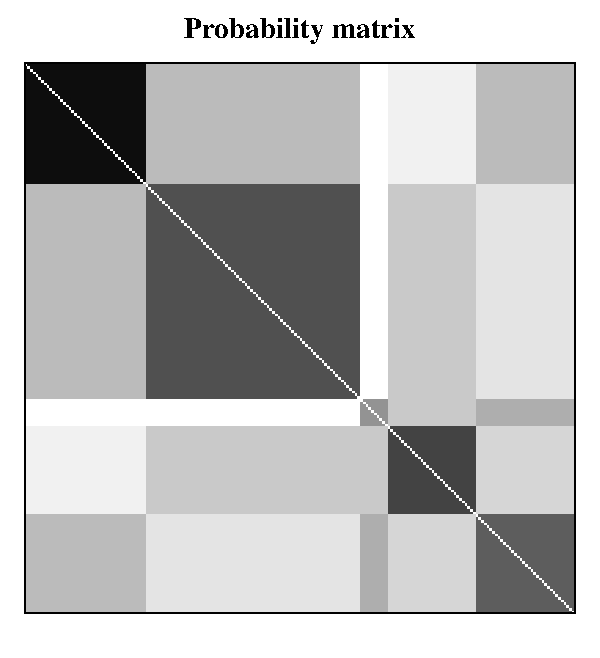
\includegraphics[height=\linewidth]{./Figures/SBM_P.pdf}
\end{subfigure}%
\begin{subfigure}{.45\textwidth}
  \centering
  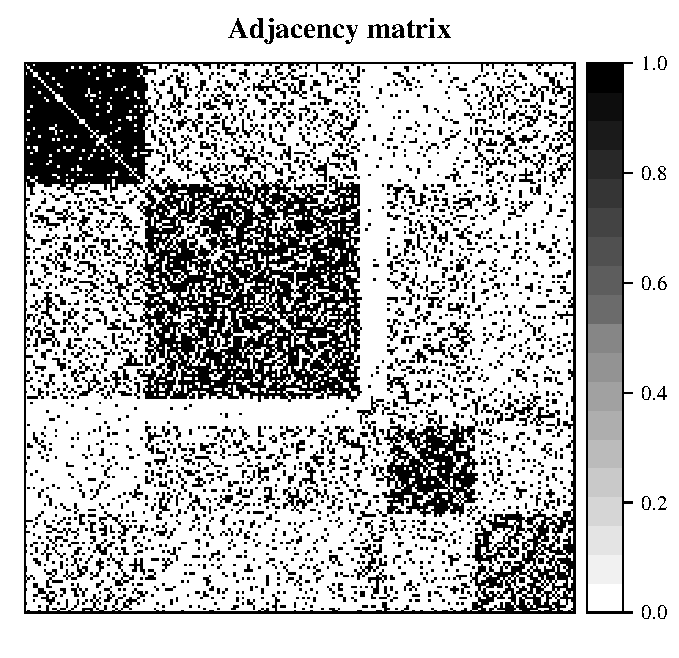
\includegraphics[height=\linewidth]{./Figures/SBM_A.pdf}
\end{subfigure}
\begin{subfigure}{.45\textwidth}
  \centering
  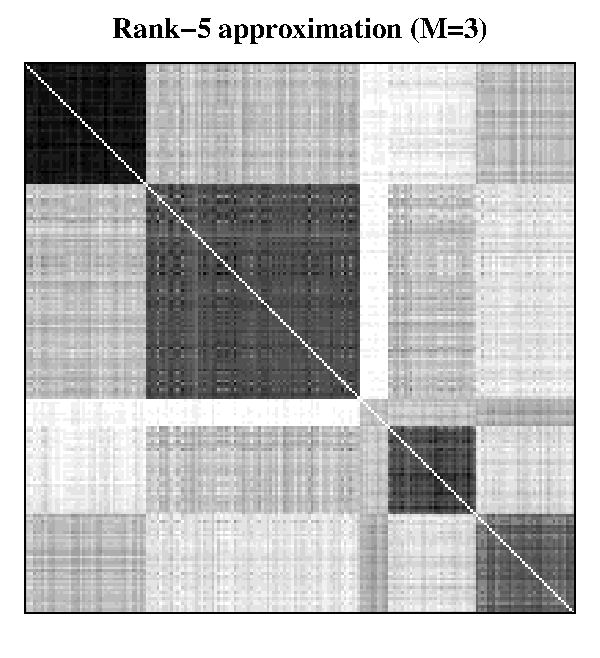
\includegraphics[height=\linewidth]{./Figures/SBM_Phat.pdf}
\end{subfigure}%
\begin{subfigure}{.45\textwidth}
  \centering
  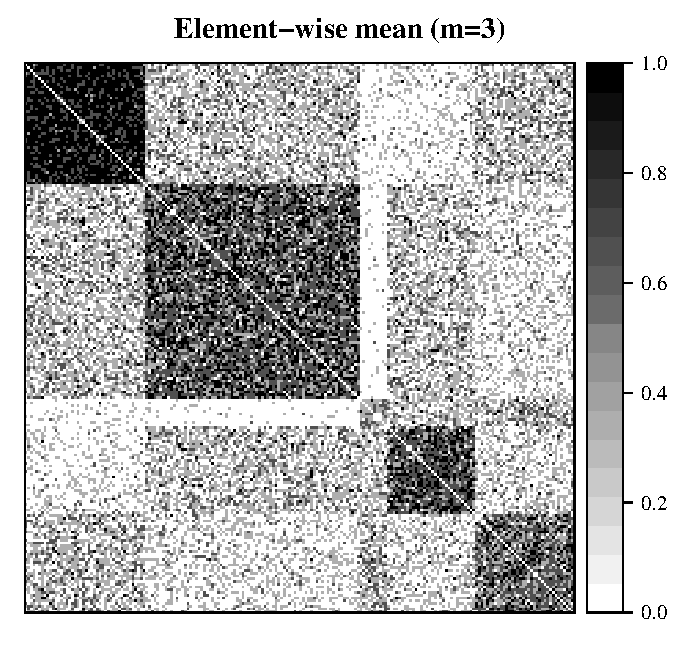
\includegraphics[height=\linewidth]{./Figures/SBM_Abar.pdf}
\end{subfigure}
\caption[Example illustrating different estimates under the stochastic blockmodel]{Example illustrating different estimates under the stochastic blockmodel.
The top left figure shows the mean graph $P$ with $K = 5$ blocks and $n=200$ vertices and the top right figure shows an adjacency matrix $A$ sampled according to the probabilities from $P$.
While $A$ is a noisy version of $P$, much of the structure of $P$ is preserved in $A$, a property we will exploit in our estimation procedure.
Based on three graphs sampled independently and identically according to the probability matrix $P$, we construct the element-wise mean $\bar{A}$, shown in the lower right panel (see Section~\ref{sec:LLG_abar}).  
Finally, by taking a rank-5 approximation of $\bar{A}$ and thresholding the values to be between $0$ and $1$, we construct our proposed estimate $\hat{P}$, shown in the lower left panel (see Section~\ref{sec:LLG_phat}).
By visual inspection, it is clear that the low-rank estimate $\hat{P}$ more closely approximates the probability matrix $P$ as compared to $\bar{A}$.
}
\label{fig:SBM_example_full}
\end{figure}








\section{Theoretical Results}
\label{sec:LLG_theoretical_result}

To estimate the mean of a collection of graphs, we consider the two estimators from Section~\ref{sec:LLG_estimator}: the entry-wise sample mean $\bar{A}$ and the low-rank $\hat{P}$ motivated by RDPG.
We evaluate our estimators in terms of mean squared error, either $\mathrm{MSE}(\hat{P}_{ij})=\Ex[\hat{P}_{ij}-P_{ij}]^2$ or $\mathrm{MSE}(\bar{A})=\Ex[\bar{A}_{ij}-P_{ij}]^2$.
While we can directly compare the difference in mean squared errors between the two estimators, it is frequently useful to consider the relative efficiency between two estimators.

\begin{definition} [Relative Efficiency]
\label{def:RE}
For two estimators $\hat{\theta}_1$ and $\hat{\theta}_2$, the {\em{relative efficiency (RE)}} between two estimators are defined as
\[
	\mathrm{RE}(\hat{\theta}_1, \hat{\theta}_2) = \frac{\mathrm{MSE}(\hat{\theta}_2)}{\mathrm{MSE}(\hat{\theta}_1)}.
\]
\end{definition}

In our case, this is $\mathrm{RE}(\bar{A}_{ij},\hat{P}_{ij}) = \frac{\mathrm{MSE}(\hat{P}_{ij})}{\mathrm{MSE}(\bar{A}_{ij})}$, with values above 1 indicating $\bar{A}$ should be preferred while values below 1 indicate $\hat{P}$ should be preferred.
Relative efficiency is a useful metric for comparing estimators because it will frequently be invariant to the scale of the noise in the problem and hence is more easily comparable across different settings.

In this section, we analyze the performance of these two estimators under the SBM by computing the entry-wise relative efficiency. 
We also consider the {\em{asymptotic relative efficiency (ARE)}}, which is the limit of the relative efficiency as the number of vertices $n \to\infty$ but with the number of graphs $m$ fixed, and the scaled relative efficiency, $n \cdot \mathrm{RE}(\bar{A}_{ij},\hat{P}_{ij}) $ which in our case normalizes the relative efficiency so that the asymptotic scaled relative efficiency is non-zero and finite. Somewhat surprisingly, we will see that the asymptotic relative efficiency will not depend on this fixed sample size $m$.

For this asymptotic framework, we assume the block memberships $\tau_i$ are drawn iid from a categorical distribution with block membership probabilities given by $\rho\in[0,1]^K$.
In particular, this implies that for each block $k$, the proportion $|\{i:\tau_i=k\}|/n$ of vertices in block $k$ will converge to $\rho_k$ as $n \to\infty$ by the law of large numbers.
We will also assume that for a given $n$, the block membership probabilities are fixed for all graphs.
Denote block probability matrix $B = \nu \nu^{\top} \in [0, 1]^{K \times K}$. 
By definition, the mean of the collection of graphs generated from this SBM is $P \in [0, 1]^{N \times N}$, where $P_{ij} = B_{\tau_i, \tau_j}$. After observing $m$ graphs on $n$ vertices $A^{(1)}, \cdots, A^{(m)}$ sampled independently from the SBM conditioned on $\tau$, we can calculate the two estimators $\bar{A}$ and $\hat{P}$.

\begin{lemma}
\label{lm:VarPhat}
For the above setting, for any $i \ne j$, if $\mathrm{rank}(B)=K=d$, we have for large enough $n$,
\[
    \Ex[(\hat{P}_{ij} - P_{ij})^2] \approx
    \frac{1/\rho_{\tau_i} + 1/\rho_{\tau_j}}{m n} P_{ij}(1-P_{ij}).
\]
And
\[
    \lim_{n \to \infty} n \cdot \mathrm{Var}(\hat{P}_{ij}) =
    \frac{1/\rho_{\tau_i} + 1/\rho_{\tau_j}}{m} P_{ij} (1 - P_{ij}).
\]
\end{lemma}
The first part of this lemma ensures that the estimator is asymptotically unbiased for $P$,
and the second part gives the form of the asymptotic variance of $\hat{P}$.

The proof of this lemma is given in Section~\ref{sec:LLG_proof} and is based on results for the variance of the adjacency spectral embedding from \citet{athreya2016limit}.
Here we provide an outline of the proof that leads to the approximate MSE of $\hat{P}$ in the stochastic blockmodel case.
The result depends on using the asymptotic results (see Theorem \ref{thm:clt_ext}) for the distribution of eigenvectors from \citet{athreya2016limit} which extend to the multiple graph setting in a straightforward way.\\
\begin{proofoutline}
The first key observation is that since $\bar{A}$ is computed from iid observations each with expectation $P$, $\bar{A}$ is unbiased for $P$ and $\mathrm{Var}(A_{ij}) = \frac{1}{m}P_{ij}(1-P_{ij})$.
The results of \citet{athreya2016limit} provide a central limit theorem for estimates of the latent position in an RDPG model for a single graph. Details of this theorem are in Theorem~\ref{thm:clt_ext}.
Since the variance of each entry is scaled by $1/m$ in $\bar{A}$, the analogous result for $\bar{A}$ is that the estimated latent positions will follow an approximately normal distribution with variance scaled by $1/m$ compared to the variance for a single graph. 

Since $\hat{P}_{ij} = \hat{X}_i^{\top} \hat{X}_j^{\phantom{\top}}$ is a noisy version of the dot product of $\nu_s^{\top} \nu_t^{\phantom{\top}}$ and each $\hat{X}_i$ is approximately independent and normal, we can use common results for the variance of the inner product of two independent multivariate normals \citep{brown1977means}.
After simplifications that occur in the stochastic blockmodel setting, we can derive that the variance of $\hat{P}_{ij}$ converges to $\left( 1/\rho_{\tau_i} + 1/\rho_{\tau_j} \right) P_{ij} (1-P_{ij})/(n \cdot m)$ as $n \to \infty$. 
Since the variance of $\bar{A}_{ij}$ is $P_{ij} (1-P_{ij})/m$, the relative efficiency between $\hat{P}_{ij}$ and $\bar{A}_{ij}$ is approximately $(\rho_{\tau_i}^{-1} + \rho_{\tau_j}^{-1})/n$ when $n$ is sufficiently large.
\end{proofoutline}

From Lemma \ref{lm:VarPhat}, we can see that the MSE of $\hat{P}_{ij}$ is of order $O(m^{-1} n^{-1})$ approximately. Similar to $\bar{A}$, the estimate will get better as the number of observations $m$ increases. Furthermore, it also benefits from a larger graph because of the use of low-rank structure. That is, $\hat{P}$ will perform better as the number of vertices of the graph $n$ increases.

Moreover, since $\bar{A}_{ij}$ is the sample mean of $m$ independent Bernoulli random variables with parameter $P_{ij}$, we have
\[
    \Ex[(\bar{A}_{ij} - P_{ij})^2] = \frac{P_{ij}(1-P_{ij})}{m}.
\]
Based on this MSE result of $\bar{A}_{ij}$ and the MSE result of $\hat{P}_{ij}$ given by Lemma \ref{lm:VarPhat}, we can conclude the following theorem naturally.
%\begin{theorem}
%\label{thm:ARE}
%In the same setting as in Lemma~\ref{lm:VarPhat}, for any $i$ and $j$, if $\mathrm{rank}(B)=K=d$, the asymptotic relative efficiency (ARE) is 
%\[
%    \mathrm{ARE}(\bar{A}_{ij}, \hat{P}_{ij}) = \lim_{N \to \infty} \mathrm{RE}(\bar{A}_{ij}, \hat{P}_{ij}) = 0.
%    \label{eq:sbm_are}
%\]
%and for large enough $N$, we have
%\begin{equation}
%	    \mathrm{RE}(\bar{A}_{ij}, \hat{P}_{ij}) \approx
%    \frac{1/\rho_{\tau_i} + 1/\rho_{\tau_j}}{N}.
%\label{eq:approx_re}
%\end{equation}
%\end{theorem}
\begin{theorem}
\label{thm:ARE}
In the same setting as in Lemma~\ref{lm:VarPhat}, for any $i \ne j$, if $\mathrm{rank}(B)=K=d$, then for large enough $n$, we have
\begin{equation}
	    \mathrm{RE}(\bar{A}_{ij}, \hat{P}_{ij}) \approx
    \frac{1/\rho_{\tau_i} + 1/\rho_{\tau_j}}{n}.
\label{eq:approx_re}
\end{equation}
And the asymptotic relative efficiency (ARE) is 
\[
    \mathrm{ARE}(\bar{A}_{ij}, \hat{P}_{ij}) = \lim_{n \to \infty} \mathrm{RE}(\bar{A}_{ij}, \hat{P}_{ij}) = 0.
    \label{eq:sbm_are}
\]
\end{theorem}
\begin{proof}
Combine the MSE result of $\bar{A}_{ij}$
\[
    \Ex[(\bar{A}_{ij} - P_{ij})^2] = \frac{P_{ij}(1-P_{ij})}{m},
\]
and Lemma \ref{lm:VarPhat}, i.e. for large enough $n$,
\[
    \Ex[(\hat{P}_{ij} - P_{ij})^2] \approx
    \frac{1/\rho_{\tau_i} + 1/\rho_{\tau_j}}{m n} P_{ij}(1-P_{ij}),
\]
we have for large enough $n$,
\[
	    \mathrm{RE}(\bar{A}_{ij}, \hat{P}_{ij}) = \frac{\mathrm{MSE}(\hat{P}_{ij})}{\mathrm{MSE}(\bar{A}_{ij})}
	    = \frac{\Ex[(\hat{P}_{ij} - P_{ij})^2]}{\Ex[(\bar{A}_{ij} - P_{ij})^2]}
	    \approx \frac{1/\rho_{\tau_i} + 1/\rho_{\tau_j}}{n}.
\]
And the ARE result follows directly by taking the limit of RE as $n \to \infty$.
\end{proof}

This theorem indicates that under the SBM, $\hat{P}$ is a much better estimate of the mean of the collection of graphs $P$ than $\bar{A}$.
Note that a relative efficiency less than 1 indicates that $\hat{P}$ should be preferred over $\bar{A}$, so under the above assumptions, as $n \to \infty$, $\hat{P}$ performs far better than $\bar{A}$.
From the result, we see that the relative efficiency is of order $O(n^{-1})$ and $n \cdot \mathrm{RE}(\bar{A}_{ij}, \hat{P}_{ij})$ converges to $1/\rho_{\tau_i}+1/\rho_{\tau_j}$ when $n \to \infty$.
An important aspect of Theorem~\ref{thm:ARE} is that the ARE does not depend on the number of graphs $m$, so the larger the graphs are, the better $\hat{P}$ is relative to $\bar{A}$, regardless of $m$.

Note that the asymptotic result here is for number of vertices going to infinity with a fixed number of graphs. Such setting is very useful in certain circumstances, for example connectomics analysis since we anticipate the collection of larger and larger brain network which will also likely initially correspond to smaller sample sizes as the technology to scale these connectome collection techniques is developed.

The approximate formula Equation~\ref{eq:approx_re} indicates that the sizes of the blocks can greatly impact the relative efficiency.
As an example, consider a 2-block SBM. 
If each of the blocks contain half the vertices, then for each pair of vertices, the relative efficiency is approximately $4/n$. 
If the first block gets larger, with $\rho_1\to 1$, then the RE for estimating $P_{ij}$ with $\tau_i=\tau_j=1$ will tend to its minimum of $2/n$. 
On the other hand as $\rho_1\to 1$, if $\tau_i=1$ and $\tau_j=2$, then since $\rho_2=1-\rho_1$, the relative efficiency for estimating such an edge pair will be approximately $1$ and the same will hold if $\tau_i=\tau_j=2$.
Note that the maximum value for the relative efficiency in a two-block model is achieved when $\rho_1=1/n$ and $\rho_2=(n-1)/n$ in which case the relative efficiency is $n/(n-1) \approx 1$.
(Note values of $\rho_s$ below $1/n$ correspond to graphs where typically no vertices are in that block, so the effective minimum we can consider for $\rho_s$ is $1/n$.)

\begin{figure}[!t]
\centering
\includegraphics[width=1\textwidth]{./Figures/Rho.pdf}
\caption[Asymptotic scaled relative efficiency in a 2-block SBM]{Asymptotic scaled relative efficiency $n \cdot \mathrm{RE}(\bar{A},\hat{P})$ in a 2-block SBM.
For each distinct pair of edge probabilities in a 2-block SBM specified in Eq.~\ref{eq:sim_setting}, the scaled relative efficiency only depends on the proportion of vertices in each block.
We show the scaled asymptotic relative efficiency as $\rho_1$ changes from $0,1$ for pairs of vertices where either both are in block one or one is in block one and one is in block two. 
These curves all intersect at a scaled relative efficiency of 4 when $\rho_1=1/2=\rho_2$.
Improvements using low-rank methods are greater for larger blocks, such as for $B_{11}$ when $\rho_1$ is close to 1, while the improvements are smaller for block pairs with relatively few vertex pairs such as $B_{11}$ when $\rho_1$ is small and $B_{12}$ when $\rho_1$ is near 0 or 1.
Note that the curve for $B_{22}$ would be the same as that for $B_{11}$ but reflected around the vertical line when $\rho_1=1/2$.
Overall, $\hat{P}$ performs best for large blocks while the improvements may be very minor for blocks with only a few vertices.}
\label{fig:RErho}
\end{figure}

To illustrate Equation~\ref{eq:approx_re} of Theorem~\ref{thm:ARE}, we consider a 2-block SBM with parameters
\begin{equation}
B = \begin{bmatrix}
0.42 & 0.2 \\
0.2 & 0.7
\end{bmatrix}
,\qquad \rho = \begin{bmatrix}
0.5 & 0.5
\end{bmatrix},
\label{eq:sim_setting}
\end{equation}
so that $|\{i:\tau_i=1\}| \approx |\{i:\tau_i=2\}|$, especially for large $n$.
Note that this simulation only focuses on the rank-2 setting primarily for the interpretability.
When calculating $\hat{P}$, we omit the dimension selection step from Algorithm~\ref{algo:LLG_basic} and instead use the true dimension $d = \mathrm{rank}(B) = 2$.
Figure~\ref{fig:RErho} shows $2/\rho_1$ and $1/\rho_1+1/\rho_2$, the scaled asymptotic RE for pairs of vertices both in block one and pairs of vertices in different blocks, respectively, in the 2-block SBM we specified earlier.
We vary $\rho_1$ between 0 and 1 to demonstrate how the number of pairs of vertices with the corresponding block memberships impacts the overall relative efficiency.
For $n=500$ and $m=100$, estimates of the scaled RE based on simulations agree very closely with their corresponding theoretical values displayed in the figure. Note that when $\rho_1 = 0.5$, the scaled RE has value $4.0$, which agrees with the result in Figure~\ref{fig:RE} for simulated data.


If instead of assuming that the graphs follow an SBM distribution, we assume the graphs are distributed according to an RDPG distribution, similar gains in relative efficiency can be realized.
While there is no compact analytical formula for the relative efficiency of $\hat{P}$ versus $\bar{A}$ in the general RDPG case, using the same ideas as in Theorem~\ref{thm:ARE}, we can show that $\mathrm{RE}(\bar{A}_{ij},\hat{P}_{ij}) = O(1/n)$.

\begin{proposition}
Suppose that $A^{(1)},A^{(2)},\dotsc,A^{(m)}$ are independently and identically distributed from an RDPG distribution with common latent positions $X_1,\dotsc,X_n$, which are independently and identically distributed from some distribution.
As the number of vertices $n \to \infty$, it holds for any $i\neq j$ that 
\[
    \mathrm{RE}(\bar{A}_{ij},\hat{P}_{ij}) = O(1/n).
\]
where again the asymptotic relative efficiency in $n$ does not depend on $m$.
\end{proposition}
The proof of this proposition closely follows the proofs of Lemma~\ref{lm:VarPhat} and Theorem~\ref{thm:ARE}, and hence we omit it here.

\begin{remark}
\label{remark:low_rank}
As we noted above, if the graphs are distributed according to an SBM or an RDPG, the relative efficiency is approximately invariant to the number of graphs $m$ when $n$ is large.
If on the other hand, the graphs are generated according to a full-rank independent edge model, then the relative efficiency can change more dramatically as $m$ changes. 
The reason for this is because for larger $m$, more of the eigenvectors of $\bar{A}$ will begin to concentrate around the eigenvectors of the mean graph.
This leads to the fact that the optimal embedding dimension for estimating the mean will increase, making $\bar{A}$ and the low-rank approximation at the optimal dimension closer together. 
As a result, $\mathrm{RE}(\bar{A},\hat{P})$ will increase as $m$ increases for full-rank models.
Indeed, for large $m$ we could have $\mathrm{RE}(\bar{A},\hat{P})\geq 1$ since we cannot guarantee that $\hat{P}$ will choose the optimal dimension.
The lack of gaps in the eigenvalues of the mean graph makes dimension reduction quite dangerous.
In an extreme case, the low-rank assumption will be most violated when all eigenvalues of the mean graph are almost equal. This leads to a certain type of structure, which is close to a constant times the identity matrix. However we do not see such structure in connectomics.
We will discuss this further in Section \ref{sec:LLG_corr_data} when applying our estimator to the CoRR dataset.
\end{remark}






\section{Finite Sample Toy Model Simulations}
\label{sec:sbm_sim}

We first illustrate the theoretical results from Section~\ref{sec:LLG_theoretical_result} regarding the relative efficiency between $\bar{A}$ and $\hat{P}$ via Monte Carlo simulation experiments in an idealized setting.
These numerical simulations will also allow us to investigate the finite sample performance of the two estimators.
Note that in Section \ref{sec:sim_iem}, we will break the model assumptions slightly and run experiment in a more realistic setting.

%\subsubsection{Simulation Setting}
Here, we consider the same 2-block SBM as in Equation~\ref{eq:sim_setting}. To be clear, we restate the parameters here:
\begin{equation*}
B = \begin{bmatrix}
0.42 & 0.2 \\
0.2 & 0.7
\end{bmatrix}
,\qquad \rho = \begin{bmatrix}
0.5 & 0.5
\end{bmatrix}.
\end{equation*}
Similarly, when calculating $\hat{P}$, we omit the dimension selection step from Algorithm~\ref{algo:LLG_basic} and instead use the true dimension $d = \mathrm{rank}(B) = 2$.

%\subsubsection{Simulation Results}
To investigate the finite sample relative efficiency, we first sample 1000 Monte Carlo replicates from the above SBM distribution with different numbers of vertices $N \in \{30, 50, 100, 250, 500, 1000 \}$ and a fixed number of graphs $m = 100$. The relative efficiency $\mathrm{RE}(\bar{A}_{ij}, \hat{P}_{ij})$ can be estimated because $P$ is known for this simulation. Since the relative efficiency only depends on the block memberships of the pair $i,j$, we estimate the relative efficiency for each block pair using
\[
    \hat{\mathrm{RE}}_{st}(\bar{A},\hat{P}) = \frac{\sum_{\tau_i=s,\tau_j=t,i \ne j} \hat{\mathrm{MSE}}(\hat{P}_{ij})}{\sum_{\tau_i=s,\tau_j=t,i \ne j} \hat{\mathrm{MSE}}(\bar{A}_{ij})}
\]
for $s,t\in\{1,2\}$, where $\hat{\mathrm{MSE}}$ denotes the estimated mean squared error based on the Monte Carlo replicates.
For the remaining simulations and real data analysis, we will always be considering estimated relative efficiency and estimated mean squared error rather than analytic results, and hence we will frequently omit that these are estimated values when it is clear from context.

In Figure~\ref{fig:RE}, we plot the (estimated) relative efficiency (top panel) and the scaled (estimated) relative efficiency (bottom panel), $n \cdot \hat{\mathrm{RE}}_{st}(\bar{A},\hat{P})$.
The different dashed lines denote the RE and scaled RE associated with different block pairs, either $B_{11}$, $B_{12}$, or $B_{22}$. 
As expected from Theorem~\ref{thm:ARE}, the top panel indicates that the relative efficiencies are all very close together and much less than 1, decreasing at the rate of $1/n$, indicating that $\hat{P}$ is performing better than $\bar{A}$.

\begin{figure}[!htbp]
\centering
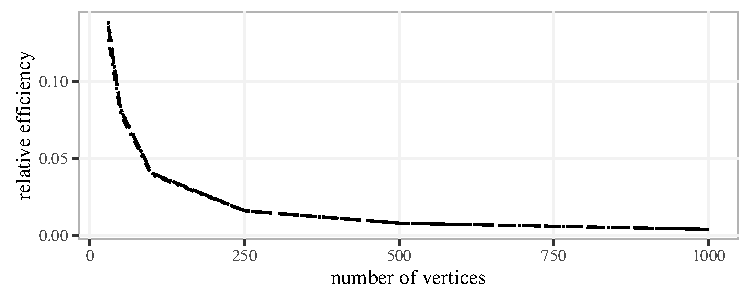
\includegraphics[width=1\textwidth]{./Figures/RE.pdf}
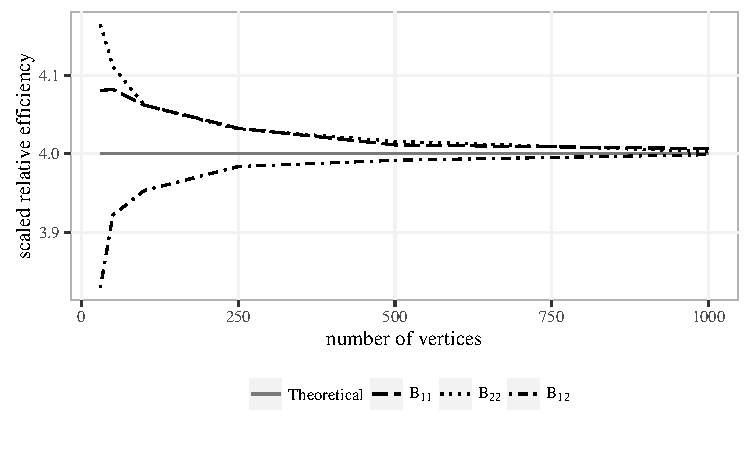
\includegraphics[width=1\textwidth]{./Figures/scaled_RE.pdf}
\caption[Finite sample relative efficiency based on simulations]{Finite sample relative efficiency based on simulations.
The top panel shows the estimated relative efficiency $\hat{\mathrm{RE}}(\bar{A},\hat{P})$ as a function of $n$ for fixed $m=100$ based on simulations of an SBM. 
For each value of $n$, we used 1000 Monte Carlo replicates of the SBM from Section~\ref{sec:sbm_sim} to estimate the RE.
Each curve corresponds to an average across vertex pairs corresponding to the three distinct block probabilities $B_{11}$, $B_{12}$, and $B_{22}$ in the two-block SBM.
Recall that values below 1 indicate that $\hat{P}$ is performing better than $\bar{A}$.
The relative efficiencies are all very close so the lines are indistinguishable. \\
To distinguish the three curves, the bottom panel shows the corresponding scaled relative efficiencies, $n \cdot \hat{\mathrm{RE}}(\bar{A},\hat{P})$.
The solid horizontal line indicates the theoretical asymptotic scaled relative which is  $1/\rho_s+1/\rho_t=4$, since $\rho_1=\rho_2=4$.
All the curves converge quickly to this theoretical limit. }
\label{fig:RE}
\end{figure}


Based on Theorem~\ref{thm:ARE}, we also have that the scaled RE converges to $1/\rho_{\tau_i}+1/\rho_{\tau_j}=4$ as $n \to\infty$ for all pairs $i,j$.
This is plotted as a solid line in the bottom panel.
From the figure, we see that $n \cdot \hat{\mathrm{RE}}_{st}(\bar{A}, \hat{P})$ converges to scaled asymptotic RE quite rapidly.
We omit error bars as the standard errors are very small for these estimates.

\begin{remark}
An intriguing aspect of these finite sample results is that the scaled relative efficiencies behave differently for small graphs with fewer vertices. 
The estimates of the edge probabilities for pairs of vertices in different blocks are much better than the estimates for edges within each block.
The reason for this is unclear and could be due to the actual values of the true probability, but it may also be due to the fact that there are approximately twice as many pairs of vertices in different blocks, $n^2/4$, than there are in the same block, $n^2/8-n/4$.
This could lead to an increase in effective sample size which may cause the larger differences displayed in the left parts of Figure~\ref{fig:RE}.
However, overall these differences are nearly indistinguishable for unscaled relative efficiency.
\end{remark}






\section{CoRR Brain Graphs Experiment}
\label{sec:LLG_corr_data}

In practice, graphs do not follow the independent edge model, let alone an RDPG or SBM, but the mean of a collection of graphs is still of interest for these cases.
To demonstrate that the estimator $\hat{P}$ is still useful in such cases, we tested its performance on structural connectomic data. 
The graphs are based on diffusion tensor MR images collected and available at the Consortium for Reliability and Reproducibility (CoRR) \citep{zuo2014open, gorgolewski2015high}.
The dataset contains 454 different brain scans, each of which was processed to yield an undirected, unweighted graph with no self-loops, using the pipeline described in \citet{roncal2013migraine} and \citet{kiar2016ndmg}.
The vertices of the graphs represent different regions in the brain defined according to an atlas.
We used three atlases, the JHU atlas with 48 vertices, the Desikan atlas with 70 vertices, and the  CPAC200 atlas with 200 vertices.
An edge exists between two vertices whenever there is at least one white-matter tract connecting the corresponding two regions of the brain. 
Details of this dataset are provided in the following section.


\subsection{Dataset Description}
\label{section:data}

The original dataset is from the Emotion and Creativity One Year Retest Dataset provided by Qiu, Zhang and Wei from Southwest University available at the Consortium for Reliability and Reproducibility (CoRR) \citep{zuo2014open, gorgolewski2015high}. It is comprised of 235 subjects, all of whom were college students. Each subject underwent two sessions of anatomical, resting state DTI scans, spaced one year apart. Due to incomplete data, only 454 scans are available.

When deriving MR connectomes, \citet{kiar2016ndmg} parcellate the brain into groups of voxels as defined by anatomical atlases. The atlases are defined either physiologically by neuroanatomists (Desikan and JHU), or are generated using an automated segmentation algorithm (CPAC200).
Once the voxels in the original image space are grouped into regions, an edge is placed between two regions when there is at least one white-matter tract, derived using a tractography algorithm, connecting the corresponding two parts of the brain.
The resulting graphs are undirected, unweighted, and have no self-loops.




\subsection{Experiment Results}

In order to evaluate the performance of the two estimators, we used a cross validation on the 454 graphs of each size. 
Specifically, for a given atlas, each Monte Carlo replicate corresponds to sampling $m$ graphs out of the 454 and computing the low-rank estimator $\hat{P}$ and the sample mean $\bar{A}$ using the $m$ selected graphs.
We then compared these estimates to the sample mean for the remaining $454-m$ adjacency matrices.
While we cannot interpret this mean graph as the probability matrix for an IEM distribution (see Section~\ref{sec:sim_iem}), the sample mean for the remaining graphs does give the proportion of times each pair of vertices are adjacent in the population from which the graphs were sampled.

While in previous sections we evaluated the mean squared error for either an individual entry or for an entire block in the SBM, in this section and the next section we will focus on the overall error for estimating the mean graph.
In particular we will use the average of the mean squared error across all pairs of vertices and we define $\mathrm{MSE}(\bar{A}) = \binom{n}{2}^{-1} \sum_{i<j}\Ex[\bar{A}_{ij}-P_{ij}]$ and similarly for $\mathrm{MSE}(\hat{P})$, which are also used for the relative efficiency.
As in the previous section, we will not use analytical evaluations of the MSE and instead estimate the MSE and relative efficiencies via Monte Carlo simulations.

We ran 1000 simulations on each of the three atlases for sample size $m=5, 10$. For $m=1$, we only have 454 different possibilities. So instead of running 1000 simulations, we looked through all 454 possible sample with size 1. As long as we determine which dimension to embed, the two estimates $\bar{A}$ and $\hat{P}$ can be calculated based on the sample.
In practice, we use algorithms like Zhu and Ghodsi's method or USVT discussed in Section~\ref{sec:dim_select} to select the dimension $d$. These methods are neither computationally advanced nor requiring sophisticated algorithms.
We plot the estimated relative efficiencies between $\bar{A}$ and $\hat{P}$ in Figure~\ref{fig:corr_re}.

\begin{figure}
\begin{center}
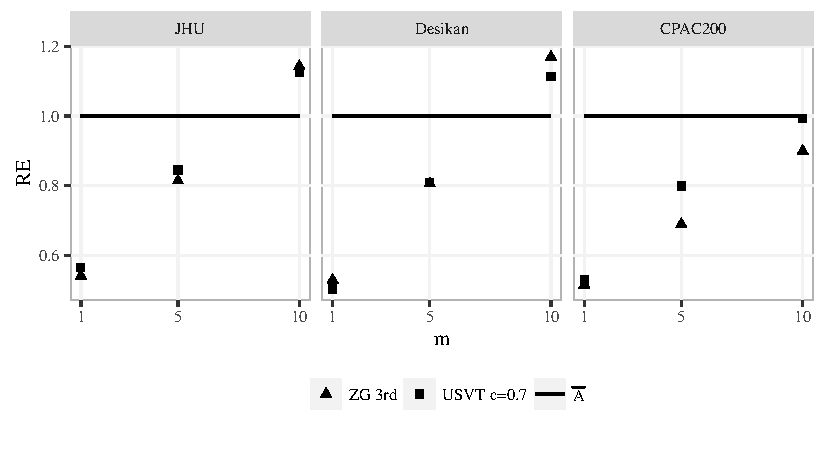
\includegraphics[width=1\linewidth]{./Figures/corr_data_REdiff.pdf}
\end{center}
\caption[Relative efficiencies of two estimators for the CoRR data set]{Relative efficiencies of $\bar{A}$ versus $\hat{P}$ for the CoRR data set.
For each atlas, JHU, Desikan, and CPAC 200, we sampled graphs which we used to compute $\bar{A}$ and $\hat{P}$.
We compared different sample sizes $m$ and different dimension selection procedures, ZG and USVT.
For each of the two methods for computing $\hat{P}$, we estimated their relative efficiencies with respect to the sample mean $\bar{A}$.
Confidence intervals all had lengths less than $0.015$, and hence we omitted them for clarity.
Overall, the relative efficiencies are greater for smaller sample sizes $m$ and larger number of vertices $n$.} 
\label{fig:corr_re}
\end{figure}

For each atlas and each sample size, we compare the Zhu and Ghodsi method \citep{zhu2006automatic} with the USVT method \citep{chatterjee2015matrix} and note that both perform reasonably well relative to the full-dimensional $\bar{A}$.
We omit confidence intervals for the estimated relative efficiencies since all confidence intervals have lengths less than $0.015$, indicating that all relative efficiencies, aside from the relative efficiency for the CPAC200 atlas at $m=10$, are very different from 1.

Again we can see that the largest improvements using $\hat{P}$ occur when $m$ is small and $n$ is large, where the RE are smaller than 1.
On the other hand, once $m=10$, $\bar{A}$ tends to do nearly as well or better than $\hat{P}$. 
Nonetheless, when applied to subgroups inference, such as all females between the age of 21 and 25, $\hat{P}$ can be really helpful for better exploring differences between groups compared to $\bar{A}$ due to a small sample size of each subgroup.
In addition, $\hat{P}$ offers certain advantages, especially since low-rank estimates can often be more easily interpretable by considering the latent position representation which will be discussed in Section~\ref{sec:interpretability}.

To further illustrate the differences between the two estimators, we considered a single random sample of size $m=5$ based on the Desikan atlas.
We calculated $\bar{A}$ and $\hat{P}$, using  Zhu and Ghodsi's 3rd elbow to select $d=11$. 
In Figure~\ref{fig:Matrix_desikan_m5}, the estimates $\bar{A}$ and $\hat{P}$ as well as the sample mean of 454 graphs (as a close estimate of $P$) are plotted in the upper level. 
Since the sample size is small, there are a lot of pairs of vertices with no edges or 5 edges in the 5 observations.
This leads to the white and black pixels in the image corresponding to $\bar{A}$.
On the other hand, $\hat{P}$ has a finer gradient of values which in this case leads to a more accurate estimate.
By calculating the mean squared error based on this sample, we can see that $\hat{P}$ (with mean squared error equals $0.015$) outperforms $\bar{A}$ (with mean squared error equals $0.016$), with a 3\% relative improvement.
In order to see where the improvements are clearly, in the upper triangular of the heat maps for $\bar{A}$ and $\hat{P}$, we highlight the edges (18 edges highlighted for $\bar{A}$ and 6 for $\hat{P}$) which have absolute estimation error larger than $0.4$.


Moreover, for the same sample discussed above, Figure~\ref{fig:Diff_desikan_m5} shows the values for the absolute estimation error $|\bar{A} - P|$ and $|\hat{P}-P|$. In addition, we include the absolute difference $|\bar{A} - \hat{P}|$ to show the overall difference between the two estimates. The lower triangular sections show the actual absolute difference while the upper triangular matrix highlights the vertex pairs with absolute differences larger than 0.4. 
There are 18 edges from $\bar{A}$ and 6 edges from $\hat{P}$ being highlighted in the figure, further indicating the superior performance of $\hat{P}$.
Note that approximately $13\%$ of all pairs of vertices are adjacent in all $454$ graphs and hence $\bar{A}$ will always have zero error for those pairs of vertices.
Nonetheless, $\hat{P}$ typically outperforms $\bar{A}$.

\begin{figure}
\begin{center}
  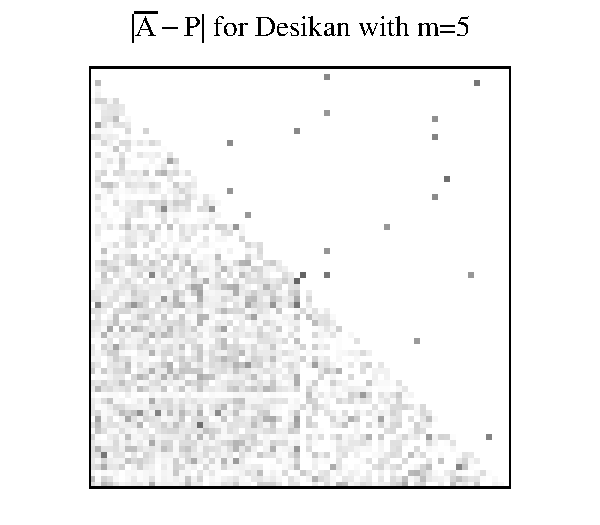
\includegraphics[height=.315\linewidth]{./Figures/Diff2_desikan_m5.pdf}\hspace{-40pt}
  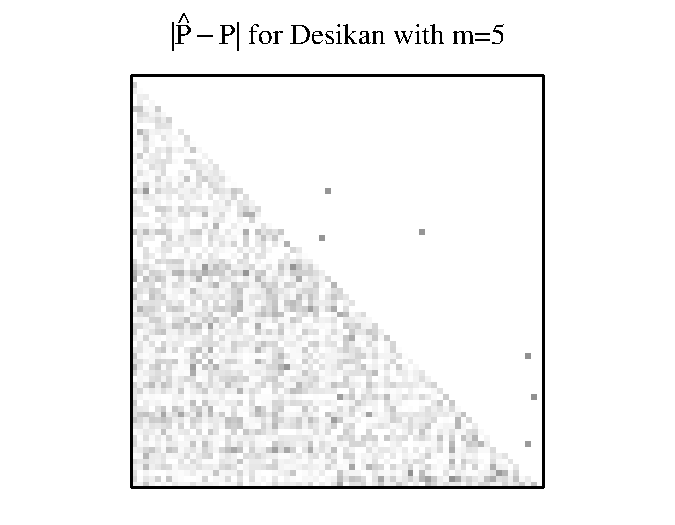
\includegraphics[height=.32\linewidth]{./Figures/Diff3_desikan_m5.pdf}\hspace{-34pt}
  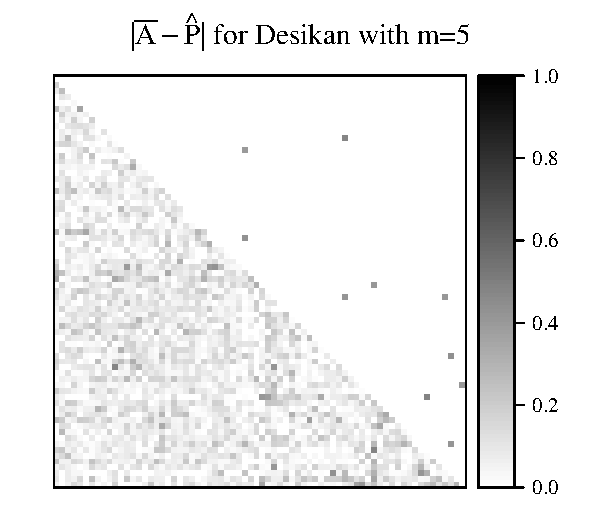
\includegraphics[height=.32\linewidth]{./Figures/Diff1_desikan_m5.pdf}
\end{center}
\caption[Heat plots of absolute estimation error for both estimators]{Heat plots of absolute estimation error for $\bar{A}$ and $\hat{P}$ (lower triangle) and absolute errors above 0.4 (upper triangle).
These heat plots show the absolute estimation error $|\bar{A} - P|$, $|\hat{P} - P|$ and $|\bar{A} - \hat{P}|$ for a sample of size $m=5$ from the Desikan dataset.
The embedding dimension for $\hat{P}$ is $d=11$ selected by the 3rd elbow of the ZG method. The lower triangular matrix shows the actual absolute difference, while the upper triangular matrix only highlights the edges with absolute differences larger than $0.4$. The fact that 18 edges from $\bar{A}$ are highlighted and only 6 edges from $\hat{P}$ are highlighted indicates that $\hat{P}$ has fewer large outliers compared to $\bar{A}$.
}
\label{fig:Diff_desikan_m5}
\end{figure}

To investigate the difference in performance with respect to the geometry of the brain, in Figure~\ref{fig:Diff_between_desikan} we plot the 50 edges with the largest differences $|\bar{A}_{ij} - P_{ij}| - |\hat{P}_{ij} - P_{ij}|$ according to the location of the corresponding regions in the brain. Red edges indicate that $\hat{P}$ overestimates $P$, while blue means that $\hat{P}$ underestimates $P$. The edge width is determined by the estimation error for $\hat{P}$, where pairs with larger estimation error are represented by thicker lines.
We also highlight the five regions corresponding to vertices that contribute most to the difference, meaning the vertices $i$ with the largest value of $\sum_j (|\bar{A}_{ij} - P_{ij}| - |\hat{P}_{ij} - P_{ij}|)$.
Notably, three of these top five regions form a contiguous group of regions.
The top five regions are the inferior temporal, middle temporal, and transverse temporal regions in the left hemisphere and the parahippocampal and parsopercularis regions in the right hemisphere of the Desikan atlas.

\begin{figure}[!htbp]
\centering
\includegraphics[width=1\textwidth]{./Figures/Diff_between_desikan.png}
\caption[Top 5 regions of the brain and top 50 connections between regions with the largest differences between two estimators]{Top 5 regions of the brain (vertices in graphs) and top 50 connections between regions (edges in graphs) with the largest differences $|\bar{A}_{ij} - P_{ij}| - |\hat{P}_{ij} - P_{ij}|$.
Red edges indicate that $\hat{P}$ overestimate $P$ while blue means that $\hat{P}$ underestimates $P$. The edge width is determined by the estimation error. Connections with larger estimation error are represented by thicker lines. This figure shows the regions and connections of the brain where $\hat{P}$ outperforms $\bar{A}$ the most for estimating $P$.}
\label{fig:Diff_between_desikan}
\end{figure}

\subsection{Exploration of Dimension Selection Procedures}

To further investigate the impact of the dimension selection procedures, we also considered all possible dimensions for $\hat{P}$ by ranging $d$ from 1 to $n$ in order to investigate the impact of the dimension selection procedures.
We plot $\hat{\mathrm{MSE}}$ of $\bar{A}$ and $\hat{P}$ in Figure~\ref{fig:LLG_realdata_MSE}.
The horizontal axis gives dimension $d$, which only impacts $\hat{P}$, which is why estimated MSE of $\bar{A}$ is shown as flat.

When $d$ is small, $\hat{P}$ underestimates the dimension and throws away important information, which leads to relatively poor performance. When $d=n$, $\hat{P}$ is equal to $\bar{A}$, so that the curve for $\hat{\mathrm{MSE}}$ for $\hat{P}$ ends at $\hat{\mathrm{MSE}}(\bar{A})$. 

In the figure, we denote the 3rd elbow found by the Zhu and Ghodsi method by a triangle, and denote the dimension selected by USVT with threshold 0.7 by a square. 
% (with largest 95\% confidence interval length to be $3.5$)
% (with largest 95\% confidence interval length to be $0.7$) 
Both dimension selection algorithms tend to select dimensions which nearly minimize the mean squared error.
% The standard error for the Zhu and Ghodsi and the USVT methods are about $0.9$ and $0.17$ respectively.

When $m$ is 1 or 5, $\bar{A}$ has large variance which leads to large $\hat{\mathrm{MSE}}$. Meanwhile, $\hat{P}$ reduces the variance by taking advantages of inherent low-rank structure of the mean graph. Such smoothing effect is especially obvious while we only have 1 observation. When $m = 1$, all weights of the graph are either 0 or 1, leading to a very bumpy estimate $\bar{A}$. In this case, $\hat{P}$ smooths the connectomes estimate and improves the performance.
Additionally, we see that there is a large range of dimensions where the performance for $\hat{P}$ is superior to $\bar{A}$. 
With a larger $m$, the performance of $\bar{A}$ improves so that its performance is frequently superior but nearly identical to $\hat{P}$.

\begin{figure}[!htbp]
\centering
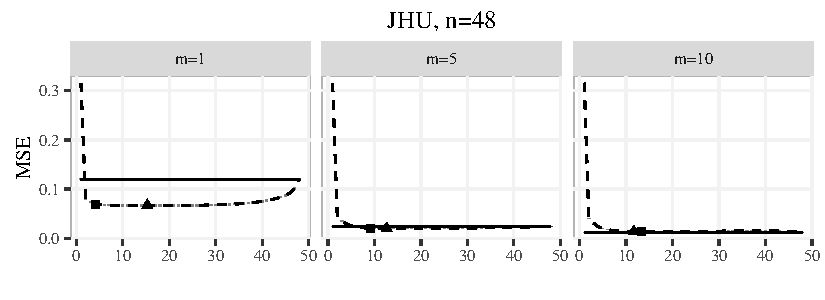
\includegraphics[width=.99\textwidth]{./Figures/corr_data_MSE_jhu.pdf}\\
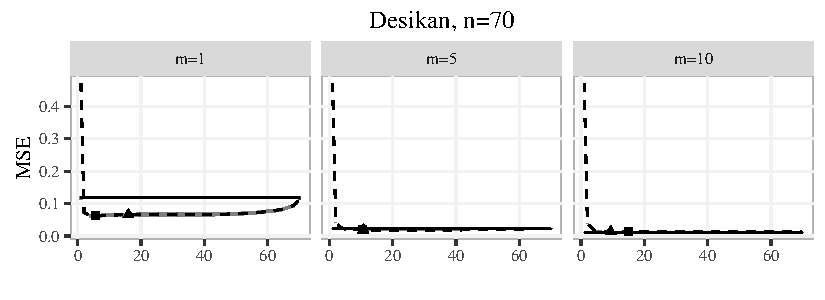
\includegraphics[width=.99\textwidth]{./Figures/corr_data_MSE_desikan.pdf}\\
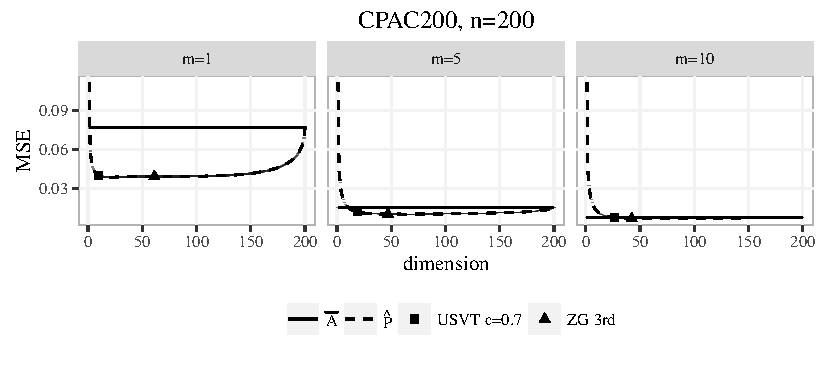
\includegraphics[width=.99\textwidth]{./Figures/corr_data_MSE_CPAC200.pdf}
\caption[Comparison of MSE of two estimators for three atlases at three sample sizes for the CoRR data]{Comparison of $\hat{\mathrm{MSE}}$ of $\hat{P}$ and $\bar{A}$ for three atlases at three sample sizes for the CoRR data.
These plots show the MSE for $\bar{A}$ (solid line) and $\hat{P}$ (dashed line) for three dataset (JHU, Desikan, and CPAC200) while embedding the graphs into different dimensions and with different sample sizes $m$. The average dimensions chosen by the 3rd elbow of Zhu and Ghodsi is denoted by a triangle
 and those chosen by USVT with threshold equaling 0.7 is denoted by a square.
Vertical intervals, visible mainly in the $n=48,70$ and $m=1$ plots, represent the 95\% confidence interval for the mean squared errors. }
\label{fig:LLG_realdata_MSE}
\end{figure}


\subsection{Interpretability of Low-rank Methods}
\label{sec:interpretability}

Low-rank methods can often be more easily interpreted in a vertexy way.
In particular, in the RDPG model, by representing a low-rank matrix in terms of the latent positions, where each vertex is represented as a vector in $\mathbb{R}^d$ and the entries of the matrix are given by the inner products of these vectors, one can analyze and visualize the geometry of these vectors in order to interpret how each vertex is behaving in the context of the larger graph. 
Now we take the CoRR brain graphs with Desikan atlases as an example. By embedding the mean graph $P$ which is the average of all 454 graphs, we get the estimated latent positions $\hat{X} \in \mathbb{R}^{n \times d}$, where $n=70$ is the number of vertices and $d = 8$ is the dimension selected by the Zhu and Ghodsi's method.
We color the brain using the first 4 dimensions of $\hat{X}$ as in Figure~\ref{fig:eigenvector_brain} respectively. By the figure of the second dimension, we can see a clear distinction of the left and right hemisphere as conveyed in the second dimension. Additionally, such a representation allows the use of techniques from multivariate analysis to further study the estimated population mean.

\begin{figure}	
\centering
\begin{subfigure}[t]{.7\textwidth}
\caption{1st dimension}
\vspace*{-16pt}
\begin{center}
  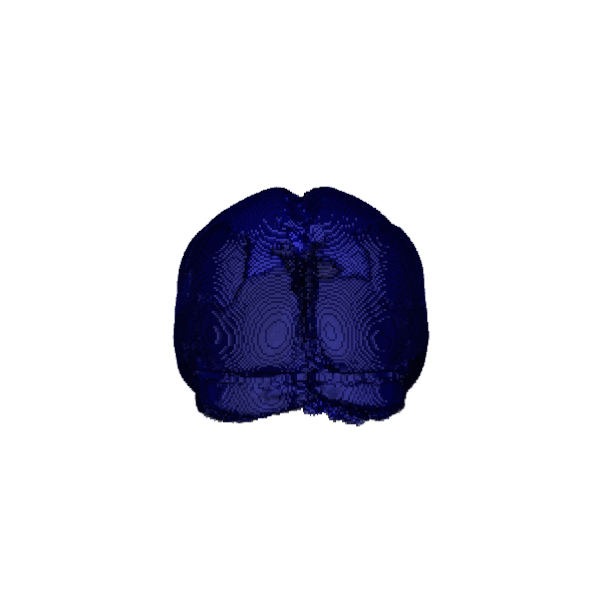
\includegraphics[trim={5cm 5cm  4cm  4cm },clip,height=.34\linewidth]{./Figures/desikan1a.png}\hspace{-9pt}
  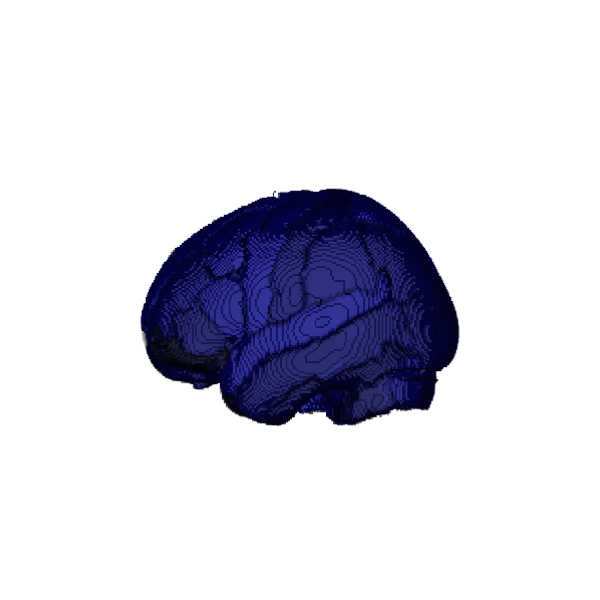
\includegraphics[trim={5cm 5cm  4cm  4cm },clip,height=.34\linewidth]{./Figures/desikan1b.png}\hspace{-9pt}
  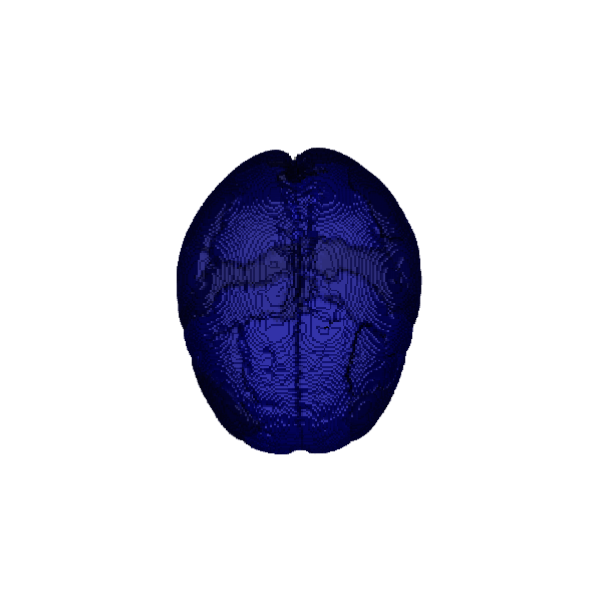
\includegraphics[trim={5cm 5cm  4cm  4cm },clip,height=.34\linewidth]{./Figures/desikan1c.png}
\end{center}
\end{subfigure}\\
\vspace*{5pt}
\begin{subfigure}[t]{.7\textwidth}
\caption{2nd dimension}
\vspace*{-16pt}
\begin{center}
  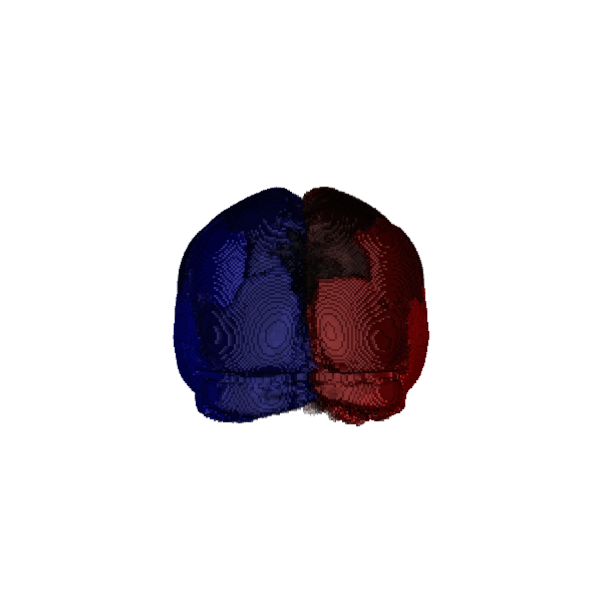
\includegraphics[trim={5cm 5cm  4cm  4cm },clip,height=.34\linewidth]{./Figures/desikan2a.png}\hspace{-10pt}
  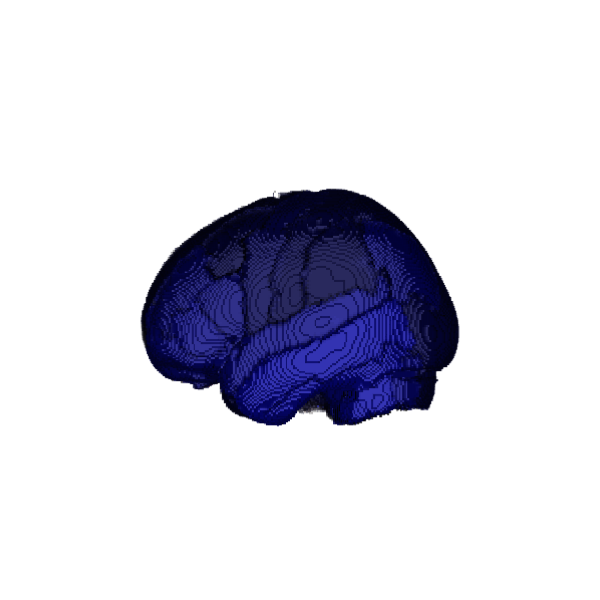
\includegraphics[trim={5cm 5cm  4cm  4cm },clip,height=.34\linewidth]{./Figures/desikan2b.png}\hspace{-10pt}
  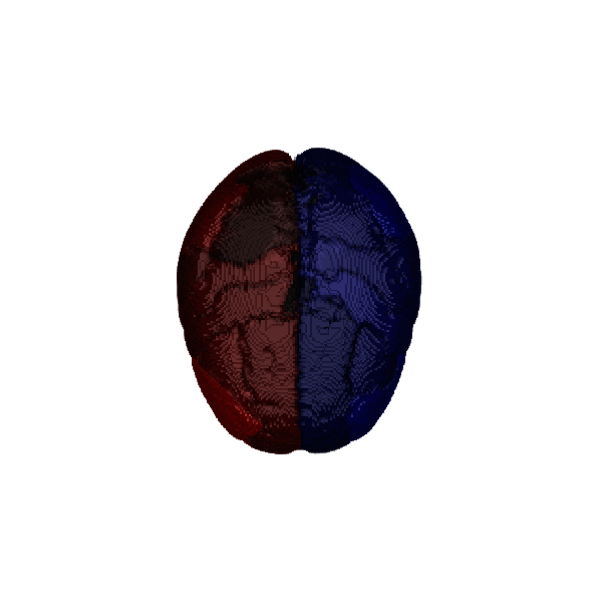
\includegraphics[trim={5cm 5cm  4cm  4cm },clip,height=.34\linewidth]{./Figures/desikan2c.png}
\end{center}
\end{subfigure}\\
\vspace*{5pt}
\begin{subfigure}[t]{.7\textwidth}
\caption{3rd dimension}
\vspace*{-16pt}
\begin{center}
  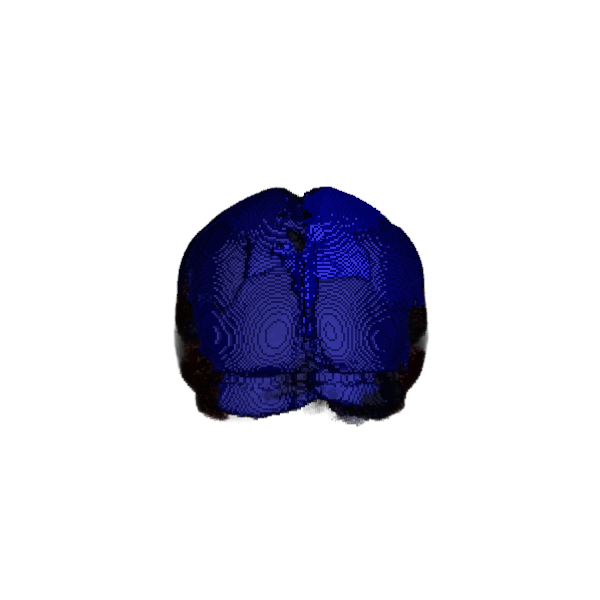
\includegraphics[trim={5cm 5cm  4cm  4cm },clip,height=.34\linewidth]{./Figures/desikan3a.png}\hspace{-10pt}
  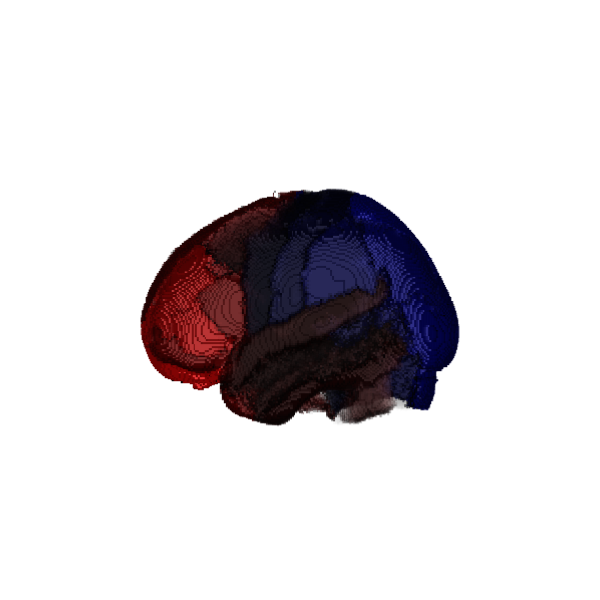
\includegraphics[trim={5cm 5cm  4cm  4cm },clip,height=.34\linewidth]{./Figures/desikan3b.png}\hspace{-10pt}
  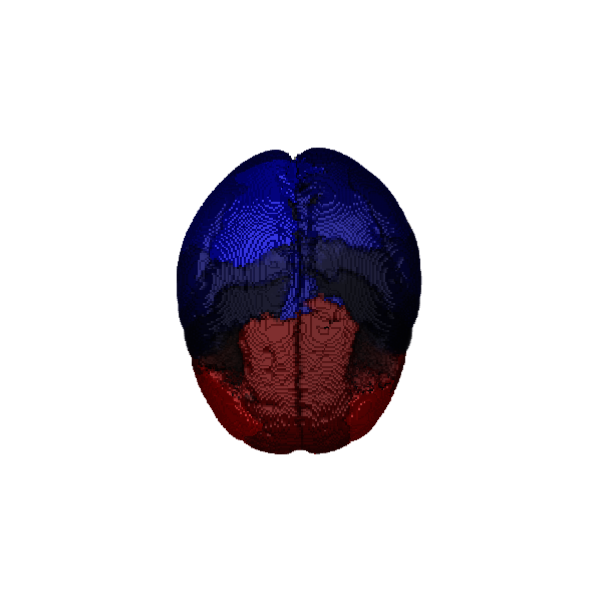
\includegraphics[trim={5cm 5cm  4cm  4cm },clip,height=.34\linewidth]{./Figures/desikan3c.png}
\end{center}
\end{subfigure}\\
\vspace*{5pt}
\begin{subfigure}[t]{.7\textwidth}
\caption{4th dimension}
\vspace*{-16pt}
\begin{center}
  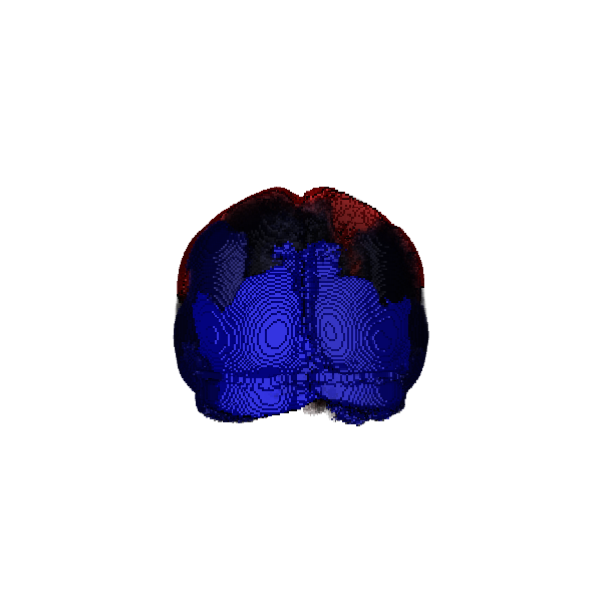
\includegraphics[trim={5cm 5cm  4cm  4cm },clip,height=.34\linewidth]{./Figures/desikan4a.png}\hspace{-10pt}
  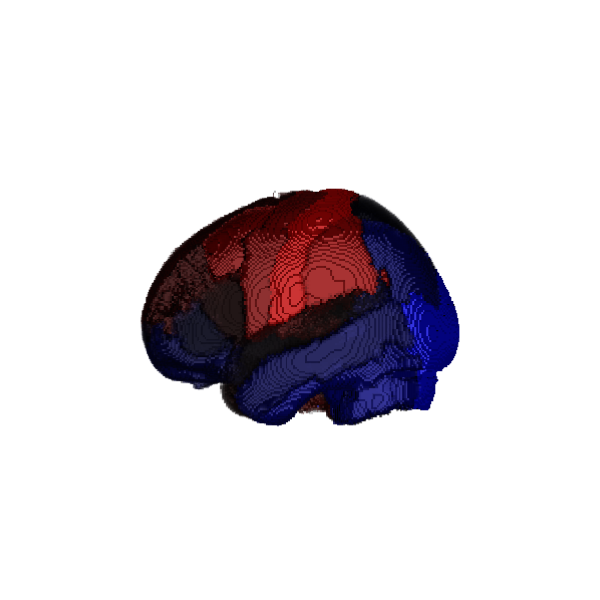
\includegraphics[trim={5cm 5cm  4cm  4cm },clip,height=.34\linewidth]{./Figures/desikan4b.png}\hspace{-10pt}
  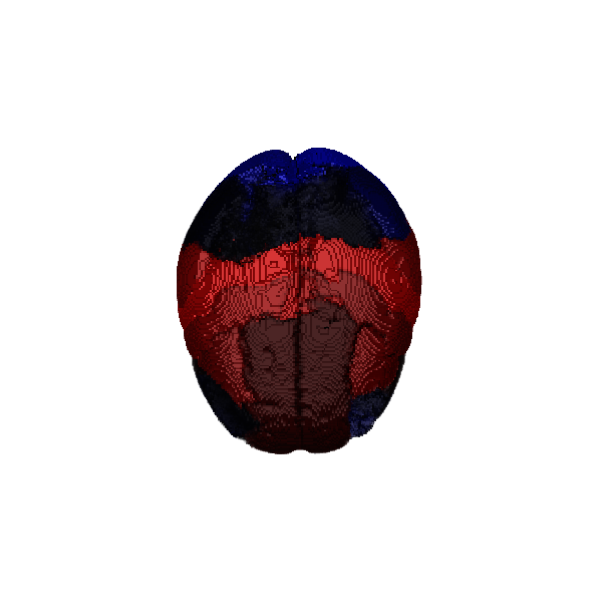
\includegraphics[trim={5cm 5cm  4cm  4cm },clip,height=.34\linewidth]{./Figures/desikan4c.png}
\end{center}
\end{subfigure}\\
\caption[Brain plots colored by the first 4 dimensions of embedding for the Desikan atlas]{Brain plots colored by the first 4 dimensions of $\hat{X}$ for the Desikan atlas respectively.
We plot the brain using the first 4 dimensions of $\hat{X}$. From the figure, we can see the embeddings have their own neuro-meaning, for example there is a clear distinction of the left and right hemisphere as conveyed in the second dimension. Also, the first dimension provides an average level of the entire brain.}
\label{fig:eigenvector_brain}
\end{figure}



\subsection{Challenges of the CoRR Dataset}

While our estimator $\hat{P}$ performs well when the sample size $m$ is small and the number of vertices $n$ is large, the CoRR dataset itself does not strictly adhere to the low-rank assumptions of our theory.

As discussed in Remark \ref{remark:low_rank}, we first check whether the dataset has the low-rank property or not. In Figure~\ref{fig:LLG_screeplot}, we plot the relative error $\|\mathrm{lowrank}_d(P)-P\|_F^2/\|P\|_F^2$ of using a rank-$d$ approximation of $P$ (see Algorithm~\ref{algo:LLG_lowrank}) as solid curves.
The rate at which this curve tends to zero provides an indication of the relative performance of using $\hat{P}_d$ as compared to $\bar{A}$ when $m$ is large. 
For all three atlases, while these error rates do tend to zero relatively quickly, substantial errors remain for any low-rank approximation.
This can be compared to the dashed lines which show how these errors would behave if $P$ was truly low-rank.
As can be expected, the CoRR dataset is actually high-rank, which violates the low-rank assumption.

\begin{figure}[!htbp]
\centering
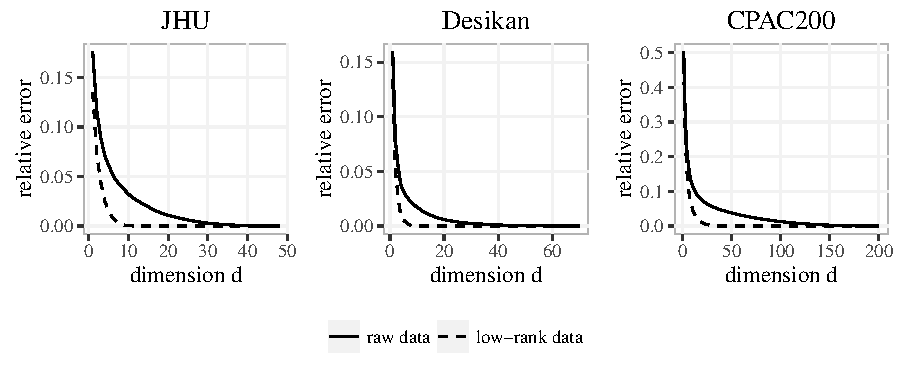
\includegraphics[width=.6\textheight]{./Figures/screeplot_ratio_all.pdf} 
\caption[Relative error of the low-rank approximation of the population mean]{Relative error of the rank-$d$ approximation of the population mean.
The solid curves show the relative error $\|\mathrm{lowrank}_d(P)-P\|_F^2/\|P\|_F^2$ of using a rank-$d$ approximation of $P$ (see Algorithm~\ref{algo:LLG_lowrank}) for three different atlases.
The relative error decays relatively slowly when $d$ is close to $n$, which indicates that $P$ is not low-rank.
Also, if $P$ actually has the low-rank property, the relative error plot will look like the dashed curves, where we revised $P$ to be low-rank by only keeping a few large eigenvalues. }
\label{fig:LLG_screeplot}
\end{figure}

In addition, by plotting the histograms of the eigenvalues of $P$ in Figure~\ref{fig:LLG_histogram}, we see that there are a bunch of negative eigenvalues, which indicates that the positive semi-definiteness is also violated in this real data experiment. This makes it even harder for $\hat{P}$ to outperform $\bar{A}$. 

 \begin{figure}[!htbp]
 \centering
 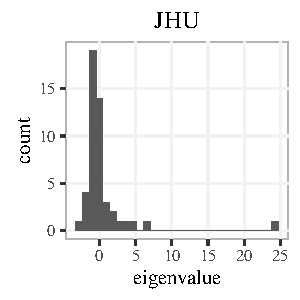
\includegraphics[height=.2\textheight]{./Figures/hist_JHU.pdf} 
 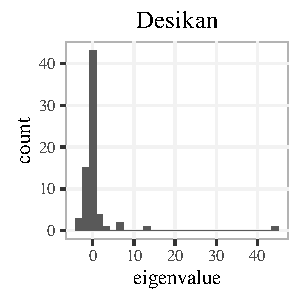
\includegraphics[height=.2\textheight]{./Figures/hist_desikan.pdf} 
 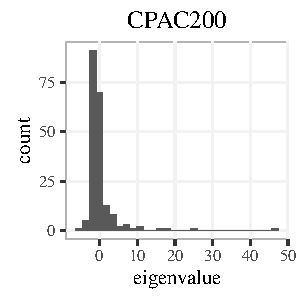
\includegraphics[height=.2\textheight]{./Figures/hist_CPAC200.pdf}
 \caption[Histogram of the population mean]{Histogram of the population mean.
 These figures show the histograms of the eigenvalues of the mean graph of all 454 graphs with diagonal augmentation. A bunch of negative eigenvalues indicate that $P$ is not positive semi-definite.
 }
 \label{fig:LLG_histogram}
 \end{figure}


Two other parts of this dataset provide challenges for our low-rank methods.
First, there are a large number of negative eigenvalues which $\hat{P}$ will not capture.
We can adapt our low-rank methods by including large negative eigenvalues as well however we found that for low sample sizes excluding negative eigenvalues improved performance.
Second, approximately 12.8\% of the entries of $P$ are exactly equal to 1.
For these edges, $\bar{A}$ will always have zero error, while $\hat{P}$ will necessarily give a less accurate estimate. 

Moreover, by the histogram of $P$, i.e. the entry-wise mean of all 454 graphs based on the Desikan atlas, as in Figure~\ref{fig:P_hist_desikan}, we can clearly see more edge probabilities are concentrated on both sides, i.e. close to 0 or 1. In particular, 12.8\% of the edges has probability equals to 1 exactly. For these edges, MLE $\bar{A}$ always recover the probability 1 exactly even with only 1 observation, while $\hat{P}$ will give a less accurate estimate because of the smoothing effect. So the CoRR dataset we consider is highly preferable to $\bar{A}$ compared to $\hat{P}$. 
However, even in this situation, $\hat{P}$ still outperforms $\bar{A}$ when the sample size is relatively small.

 \begin{figure}[!htbp]
 \centering
 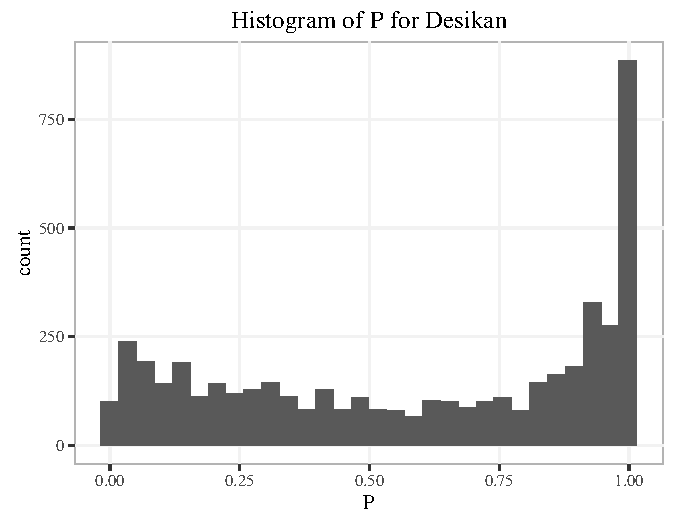
\includegraphics[width=0.8\textwidth]{./Figures/P_hist_desikan.pdf}
 \caption[Histogram of mean graph for Desikan atlas]{Histogram of $P$ for Desikan atlas.
 This figure shows the histogram of $P$, i.e. the entry-wise mean of all 454 graphs based on the Desikan atlas. More edge probabilities of $P$ are concentrated on both sides, i.e. close to 0 or 1. In particular, 12.8\% of the edges has probability equals to 1 exactly.}
 \label{fig:P_hist_desikan}
 \end{figure}

Despite all these challenges, our results show that when the sample size is relatively small, such as $m=1$ or $m=5$, and for the atlases with a larger number of vertices, $\hat{P}$ still gives a better estimate than $\bar{A}$ for the CoRR dataset.
Importantly, this improvement is robust to the embedding dimension provided the dimension is not underestimated.



\subsection{Lobe Structure behind the Low-rank Methods}
\label{section:lobe_structure}
In previous sections, we have shown that how the low-rank methods help us improve the accuracy of estimation while providing convenient interpretations simultaneously. Certainly there is more behind it. In this section, we focus on the lobe structure in particular.

The lobes of the brain is an anatomical classification, which has been shown to be related to different brain functions. Basically, there are 4 different lobes for each hemisphere, i.e. Frontal, Parietal, Occipital, and Temporal.
For the Desikan atlas, there are 70 different regions (35 regions for each hemisphere). Each region belongs to one lobe. However, 8 regions of the Desikan atlas (Unknown, Banks of Superior Temporal Sulcus, and Corpus Callosum, for both hemispheres) do not have obvious lobe assignment. So we cluster them into a new lobe category named ``other'' to resolve this issue.

Generally, the regions within the same lobe should be more similar compared to the regions across the lobes. In order to see whether the embedded latent positions $X$ preserve this property or not, we propose a test statistics $T$ to be the average differences between vertices within the same lobe minus the average differences between vertices across different lobes, i.e.
\[
T(X, l) = \frac{\sum_{i \ne j, l(i) = l(j)} \|X_i - X_j \|_2}{\sum_{i \ne j, l(i) = l(j)} 1} -
\frac{\sum_{i \ne j, l(i) \ne l(j)} \|X_i - X_j \|_2}{\sum_{i \ne j, l(i) \ne l(j)} 1},
\]
where $l(i)$ represents the lobe assignment for vertex $i$. If the latent positions $X$ and the lobe assignment $l$ are independent, then we expect $T(X, l)$ to be close to zero. A small test statistic $T(X, l)$ indicates that latent positions of the regions within the same lobe are closer compared to the ones across the lobes, which is evidence that the low-rank methods preserves the lobe structure.

However, the anatomical geometry might contribute to the dependence between $X$ and $l$ and we do not want to be distracted by this factor. So instead of testing the dependence between $X$ and $l$, we are more interested in the following hypothesis test:

$H_0$: $X$ and $l$ are conditionally independent given anatomical geometry.

$H_A$: $X$ and $l$ are conditionally dependent given anatomical geometry.

In this situation, we can focus on how much of the lobe structure is really captured by the low-rank methods without affected by the inherent spatial relationship. Note that this test is significantly underpowered compared to the test on a unconditional independence.
To test under the anatomical geometry conditions, we permute the lobe assignment $l$ in a way that the number of regions in each lobe remain the same and the regions within the same lobe are still spatially connected. In order to permute under such constraints, we define a flip to be a swap of two pairs of vertices which keeps the number of regions in each lobe, and do it several times.

As mentioned before, there are 10 lobes and 70 regions based on the Desikan atlas. 
We say two regions are adjacent if they share a common boundary. We denote such spatial adjacency by an adjacency matrix $S$ for the 70 regions, where $S_{ij} = 1$ means region $i$ and region $j$ are contain a pair of voxels, $v_i$ and $v_j$, which are spatially adjacent.
If this is true, then we say region $j$ is a neighbor of region $i$.
We denote the lobe i.d. for region $i$ by $l_i$.

Now we define a uniform $1$-flip to be:
\begin{enumerate}
\item Select a pair of adjacent regions (region $i_1$ and region $j_1$) across the boundary of lobes uniformly, i.e. $S_{i_1 j_1} = 1$ and $l(i_1) \ne l(j_1)$;
\item Uniformly select another pair of adjacent regions (region $i_2$ and region $j_2$ where $i_1 \ne i_2$ and $j_1 \ne j_2$) across the same boundary of lobes uniformly, i.e. $S_{i_2 j_2} = 1$ and $l(i_1) = l(i_2)$ and $l(j_1) = l(j_2)$;
\item Reassign region $j_1$ to lobe $l_{i_1}$ and reassign region $i_2$ to lobe $l_{j_2}$.
\end{enumerate}

By the definition, after a uniform $1$-flip, the number of regions in each lobe stays the same, where only two regions are changed to a different lobe.

Then we can define a uniform $k$-flip naturally as sequentially performing uniform $1$-flip $k$ times.
Note that after a uniform $k$-flip, the number of regions in each lobe still keeps the same.

In the permutation test, we apply a uniform $k$-flip and calculate the test statistic $T(X, l)$ based on the lobe assignment after flipping.
The $p$-value is computed as the proportion of uniform $k$-flips with a $T$ value smaller than the $T$ value for the true lobe assignments.


For a fixed number of flips, we ran 1000 simulations and calculate the test statistics $T(X, l)$ after the permutation. We vary the number of flips from 1 to 10 and the results are shown in Figure~\ref{fig:violin_plot}. In this violin plot, we use dashed line to represent the $T(X, l)$ based on the true lobe assignment. As the number of flips increases, $T(X, l)$ converges to the expected value under the assumption that $X$ and $l$ are independent in a constrained way mentioned above. And we can see that the $T(X, l)$ according to the true lobe assignment move away from the 95\% confidence interval. We also calculate the corresponding p-values and labeled them in the figure. We can see that when the number of flips is larger than 7, the p-value is less than 0.05, which suggests that the latent positions based on the low-rank methods preserves the lobe structure regardless of the anatomical geometry.

\begin{figure}[!htbp]
\centering
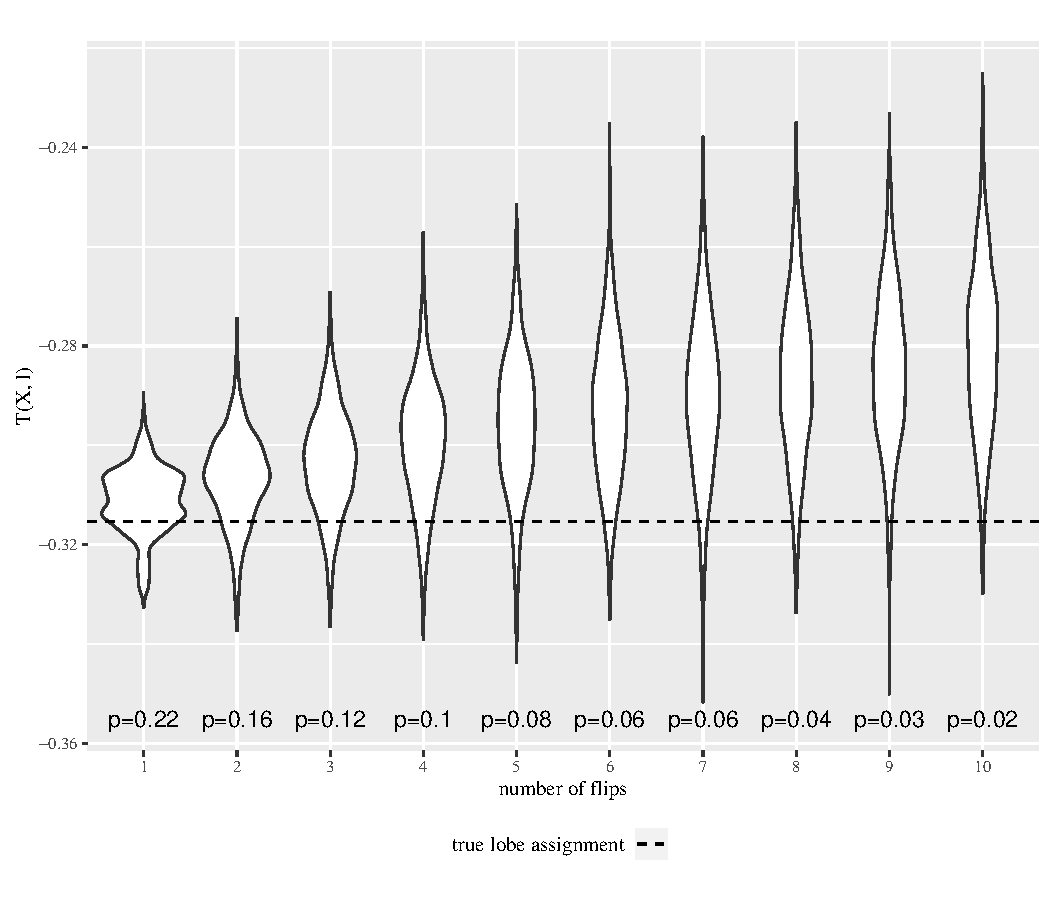
\includegraphics[width=1\textwidth]{./Figures/violinplot_new_flip_2norm_1_8.pdf}
\caption[Violin plot of the permutation test]{Violin plot of the permutation test.
We run 1000 simulations for each number of flips. Dashed line represents the situation based on true lobe assignment. As the number of flips increases, $T(X, l)$ converges to the expected value under the assumption that $X$ and $l$ are independent in a constrained way mentioned above. And we can see that the $T(X, l)$ according to the true lobe assignment move away from the 95\% confidence interval.}
\label{fig:violin_plot}
\end{figure}

%\begin{figure}[!htbp]
%\centering
%\includegraphics[width=0.8\textwidth]{pvalue_new_flip_2norm_1_8.pdf}
%\caption{{\bf P-value of the permutation test.}
%This figure shows the p-value of the permutation test based on different number of flips. When the number of flips is larger than 7, the p-value is less than 0.5, which suggests that the latent positions based on the low-rank methods preserves the lobe structure.}
%\label{fig:pvalue}
%\end{figure}





%\begin{figure}[!htbp]
%\centering
%\includegraphics[width=1\textwidth]{JHU.png}
%\caption{Comparison of MSE between $\bar{A}$ (solid line) and $\hat{P}$ (dashed line) for JHU dataset while embedding the graphs into different dimensions with different size $M$ of the subsamples. The dimension chosen by the 3rd elbow of Zhu and Ghodsi is denoted in triangle, and chosen by USVT with threshold equals 0.7 is denoted in square. Vertical intervals represent the 95\% confidence interval. When $M$ is small, $\hat{P}$ outperforms $\bar{A}$ with a flexible range of the embedding dimension including what Zhu and Ghodsi selects.}
%\label{fig:JHU}
%\end{figure}
%
%\begin{figure}[!htbp]
%\centering
%\includegraphics[width=1\textwidth]{desikan.png}
%\caption{Comparison of MSE between $\bar{A}$ (solid line) and $\hat{P}$ (dashed line) for desikan dataset while embedding the graphs into different dimensions with different size $M$ of the subsamples. The dimension chosen by the 3rd elbow of Zhu and Ghodsi is denoted in triangle, and chosen by USVT with threshold equals 0.7 is denoted in square.  Vertical intervals represent the 95\% confidence interval.  When $M$ is small, $\hat{P}$ outperforms $\bar{A}$ with a flexible range of the embedding dimension including what Zhu and Ghodsi selects.}
%\label{fig:desikan}
%\end{figure}
%
%\begin{figure}[!htbp]
%\centering
%\includegraphics[width=1\textwidth]{CPAC200.png}
%\caption{Comparison of MSE between $\bar{A}$ (solid line) and $\hat{P}$ (dashed line) for CPAC200 dataset while embedding the graphs into different dimensions with different size $M$ of the subsamples. The dimension chosen by the 3rd elbow of Zhu and Ghodsi is denoted in triangle, and chosen by USVT with threshold equals 0.7 is denoted in square.  Vertical intervals represent the 95\% confidence interval.  When $M$ is small, $\hat{P}$ outperforms $\bar{A}$ with a flexible range of the embedding dimension including what Zhu and Ghodsi selects.}
%\label{fig:CPAC200}
%\end{figure}
%
%\begin{figure}
%\centering
%\begin{subfigure}{.33\textwidth}
%  \centering
%  \includegraphics[width=1.2\linewidth]{P_JHU.png}
%\end{subfigure}%
%\begin{subfigure}{.33\textwidth}
%  \centering
%  \includegraphics[width=1.2\linewidth]{Abar_JHU_m5.png}
%\end{subfigure}
%\begin{subfigure}{.33\textwidth}
%  \centering
%  \includegraphics[width=1.2\linewidth]{Phat_JHU_m5.png}
%\end{subfigure}
%\caption{Comparison between the mean of 454 graphs $P$ and two estimates $\bar{A}$ and $\hat{P}$ derived from a sample of size $M=5$ from JHU dataset while embedding the graphs into dimension $d=15$ selected by the 3rd elbow of ZG method.}
%\label{fig:adj_JHU_m5}
%\end{figure}
%
%\begin{figure}[!htbp]
%\centering
%\includegraphics[width=1\textwidth]{Vertex_Diff_Phat_desikan.png}
%\caption{Top 5 regions of the brain (vertices in graphs) with largest absolute difference $|\hat{P} - P|$.}
%\label{fig:Vertex_Diff_Phat_desikan}
%\end{figure}
%
%\begin{figure}[!htbp]
%\centering
%\includegraphics[width=1\textwidth]{Edge_Diff_Phat_desikan.png}
%\caption{Top 1\% (49) connections between regions (edges in graphs) with largest absolute difference $|\hat{P} - P|$.}
%\label{fig:Vertex_Diff_Phat_desikan}
%\end{figure}








\section{Synthetic Data Analysis for Full Rank IEM}
\label{sec:sim_iem}

While the theory we have developed is based on the assumption that the mean graph is low rank, as we have seen in Section~\ref{sec:LLG_corr_data}, $\hat{P}$ often performs well even when this assumption is false. 
To further illuminate this point, we performed a synthetic data analysis under a full-rank independent edge model where we used the sample mean of the 454 graphs in the Desikan dataset as the probability matrix $P$.
As in the previous section, we simulated datasets from the full rank IEM distribution with probability matrix $P$ of size $m=1,5$, and $10$ and used $\bar{A}$ and $\hat{P}$, where we varied the rank of $\hat{P}$ from $1$ to $70$.

Figure~\ref{fig:sim_desikan} shows the resulting estimated MSE for $\bar{A}$ (solid line) and $\hat{P}$ (dashed line) for simulated data based on the full rank probability matrix $P$ shown in the left panel of Figure~\ref{fig:Matrix_desikan_m5}.
We see that the results are very similar to those presented in Section~\ref{sec:LLG_corr_data}, though overall $\hat{P}$ performs even better than in the real data experiments. 
When $m$ is small, $\hat{P}$ outperforms $\bar{A}$ with a flexible range of the embedding dimension including those selected by the Zhu and Ghodsi method.
On the other hand, when $m$ is large enough, both estimators perform well with the decision between the two being less conclusive.
This simulation again shows the robustness of $\hat{P}$ to deviations from the RDPG model, specifically if the probability matrix is full-rank.

We also note that the finite-sample relative efficiency in these cases shows is even more favorable to $\hat{P}$, with relative efficiencies lower than $1/3$ for $m=1$, than for the real data, where relative efficiencies were at best around $1/2$ for $m=1$.
From this observation, we can postulate that the degradation in the performance of $\hat{P}$ in real data can at least partially be attributed to the fact that the independent edge assumption does not hold for real data.


\begin{figure}[!htbp]
\centering
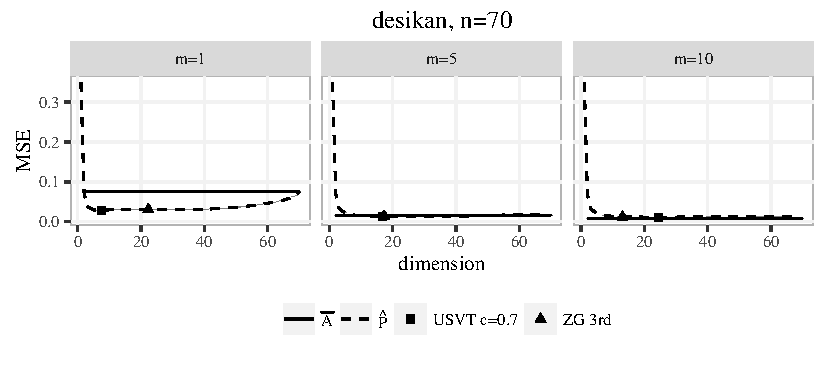
\includegraphics[width=1\textwidth]{./Figures/sim_desikan.pdf}
\caption[Comparison of two estimators for synthetic data analysis]{Comparison of $\hat{P}$ and $\bar{A}$ for synthetic data analysis.
As in Figure~\ref{fig:RE}, this figure shows $\hat{\mathrm{MSE}}$ for $\bar{A}$ (solid line) and $\hat{P}$ (dashed line) for simulated data with different sample sizes $m$ based on the sample mean for the Desikan dataset. Again, the average of dimensions selected by the USVT method (square) and the ZG method (triangle) tend to nearly approximate the optimal dimension. 
Overall, we see that the structure of these plots well approximates the structure for the real data indicating that performance for the independent edge model will tend to translate in structure to non-independent edge scenarios. 
On the other hand, the relative efficiency $\hat{\mathrm{RE}}(\bar{A},\hat{P})$ is lower for this synthetic data analysis than for the CoRR data.}
\label{fig:sim_desikan}
\end{figure}




%\section{Discussion}
%\label{sec:LLG_discussion}
%
%Motivated by the RDPG model, in this chapter, our methodology takes advantage of the low-rank structure of the graphs by applying low-rank approximation to the entry-wise MLE. 
%We give a closed form for the asymptotic relative efficiency between the entry-wise MLE $\bar{A}$ and our estimator $\hat{P}$ in the case of a stochastic blockmodel, demonstrating that when the number of vertices $N$ is sufficiently large, low-rank methods provide a substantial improvement.
%In particular, we show that for a stochastic blockmodel with fixed number of blocks $K$, block size proportion $\rho$, and number of graphs $m$, the low-rank estimator $\hat{P}$ has MSE which is on the order of $n$ times lower than the MSE for $\bar{A}$.
%
%Moreover, our estimator outperforms the entry-wise MLE in a cross validation analysis of the CoRR brain graphs and in low- and full-rank simulation settings.
%These results illustrate that $\hat{P}$ performs well even when the low-rank assumption is violated and that $\hat{P}$ is robust and can be applied in practice.
%
%One of the key observations from our real data analysis was that the largest improvements using the low-rank method occurred when the number of graphs $m$ was small, and that it provided only minor improvements or even degraded performance slightly when $m$ was large. 
%However, even in large scale studies the low-rank methods will be useful for estimating graph means for subpopulations, e.g. the population of females over 60 with some college education.
%Using the element-wise sample mean for such small strata, which may have fewer than ten subjects, will frequently result in a degradation of performance.
%Similarly, \citet{durante2014nonparametric} used low-rank deviations from a full rank population mean to model collections of graphs and our methods could be easily adapted to those ideas.
%
%While the low-rank methods considered in this paper will often offer substantial improvements, further refinements of these methods which account for the particular traits of connectomics data would be useful to improve estimation further.
%For example, we assume that the adjacency matrix is observed without contamination, however in practice there will be noise in the observed graph and one may seek to account for this noise with more robust methods.
%This may be especially fruitful when each graph has weighted edges and the weights themselves have noisy or heavy-tailed distributions.
%Rank-based methods and robust likelihood methods could be very useful in that case \citep{huber2009robust,qin2013maximum}. 
%
%Another issue that arose in our analysis of the connectome dataset was the presence of structural ones in the mean graph for the population. 
%These structural ones appear since edges between certain regions of the brain are present in all or nearly all members of the healthy population. 
%The low-rank methods tend to miss these always-present edges while the sample mean will always capture them.
%Detecting and incorporating structural ones and zeros could yield methods that share the best elements of both methods considered here.
%
%For the CoRR dataset, we used a cross-validation framework where we compared the estimates based on a subsample to the mean for the held-out set. 
%Another option would be to compare the estimates $\bar{A}$ and $\hat{P}$ to the mean for the entire population including the subsample.
%Both of these analyses lead to very similar results in the cases presented above, but for various reasons one may prefer one analysis over another.
%The cross-validation method is most reasonable from a prediction perspective where prediction about new samples is of interest.
%If instead one is interested in learning directly about the mean of a population, especially a finite population, the sub-sampling approach may be the most logical choice.






\section{Appendix: Proofs for Theory Results}
\label{sec:LLG_proof}

Here we present the proofs of the results in Section~\ref{sec:LLG_theoretical_result}. To keep the ideas clear and concise, we leave out some details which are only slight changes to previous works.
We assume the block memberships $\tau_i$ are drawn iid from a categorical distribution with block membership probabilities given by $\rho\in[0,1]^K$ where $\sum_i \rho_i =1$.
We will also assume that for a given $n$, the block memberships are fixed for all graphs.

Denote matrix of between-block edge probabilities by $B = \nu \nu^{\top} \in[0,1]^{K\times K}$ which we assume has rank $K$ and is positive definite. 
By definition, the mean of the collection of graphs generated from this SBM is $P$, where $P_{ij} = B_{\tau_i, \tau_j}$. 

We observe $m$ graphs on $n$ vertices $A^{(1)}, \cdots, A^{(m)}$ sampled independently from the SBM conditioned on $\tau$.
Define $\bar{A} = \frac{1}{m} \sum_{t=1}^m A^{(t)}$. Let $\hat{U} \hat{S} \hat{U}^{\top}$ be the best rank-$d$ positive semidefinite approximation of $\bar{A}$, then we define $\hat{P} = \hat{X} \hat{X}^{\top}$, where $\hat{X} = \hat{U} \hat{S}^{1/2}$.

The proofs presented here will rely on a central limit theorem developed in \citet{athreya2016limit}. 
We modify the theorem slightly to account for the multiple graph setting and present it in the special case of the stochastic blockmodel.

\begin{theorem}[Corrolary of Theorem 1 in \citet{athreya2016limit}]
\label{thm:clt_ext}
  In the setting above, let $X=[X_1,\dotsc,X_n]^{\top} \in \mathbb{R}^{K \times d}$ have row $i$ equal to $X_i=\nu_{\tau_i}$ (recall that $\tau_i$ are drawn from $[K]$ according to the probabilities $\rho$).
	Then there exists an orthogonal matrix $W$ such that for each row $i$ and $j$ and any $z \in \mathbb{R}^{d}$, conditioned on $\tau_i=s$ and $\tau_j=t$,
  \begin{equation}
    \label{eq:4}
    \mathbb{P}\left\{\sqrt{n}( W \hat{X}_i - \nu_s ) \leq z, \sqrt{n}( W \hat{X}_j - \nu_t) \leq z'\right\}
=  \Phi(z, \Sigma(\nu_s)/m)  \Phi(z', \Sigma(\nu_t)/m) +o(1)
  \end{equation}
  where $\Sigma(x) =\Delta^{-1}\Ex[ X_j X_j^\top(x^\top X_j -(x^\top
  X_j)^2)]\Delta^{-1}$ and $\Delta=\Ex[ X_1 X_{1}^{T}]$ is the second
  moment matrix, with all expectations taken unconditionally.
  The function $\Phi$ is the cumulative distribution function for a multivariate normal with mean zero and the specified covariance, and $o(1)$ denotes a function that tends to zero as $n \to \infty$.
\end{theorem}
The proof of this result follows very closely the proof of the result in the original paper with only slight modifications for the multiple graph setting.

We now prove a technical lemma which yields the simplified form for the variance under the stochastic blockmodel.

\begin{lemma}
\label{lm:mseForm}
In the same setting as Theorem~\ref{thm:ARE}, for any $1 \le s, t \le K$, we have
\[
	\nu_s^{\top} \Sigma(\nu_t) \nu_s^{\phantom{\top}} = \frac{1}{\rho_s} \nu_s^{\top} \nu_t^{\phantom{\top}} (1- \nu_s^{\top} \nu_t).
\]
\end{lemma}
\begin{proof}
Under the stochastic blockmodel with parameters $(B, \rho)$, we have $X_i \stackrel{iid}{\sim} \sum_{k=1}^K \rho_k \delta_{\nu_k}$, where $\nu = [\nu_1, \cdots, \nu_K]^{\top}$ satisfies $B = \nu \nu^{\top}$. Without loss of generality, we could assume that $\nu = U S$ where $U = [u_1, \cdots, u_K]^{\top}$ is orthonormal in columns and $S$ is a diagonal matrix. Here we can conclude that $\nu_s^{\top} = u_s^{\top} S$. Defining $R = \text{diag}(\rho_1, \cdots, \rho_K)$, we have
\[
	\Delta = \Ex[X_1 X_1^{\top}] = \sum_{k=1}^K \rho_k \nu_k \nu_k^{\top} = \nu^{\top} R \nu = S U^{\top} R U S.
\]
Thus
\begin{align*}
	\nu_s^{\top} \Sigma(\nu_t) \nu_s = &
    \nu_s^{\top} \Delta^{-1} \sum_{k=1}^K \rho_k \nu_k \nu_k^{\top} (\nu_t^{\top} \nu_k)(1 - \nu_t^{\top} \nu_k) \Delta^{-1} \nu_s \\
    = & \sum_{k=1}^K \rho_k (\nu_s^{\top} \Delta^{-1} \nu_k) (\nu_k^{\top} \Delta^{-1} \nu_s) (\nu_t^{\top} \nu_k) (1 - \nu_t^{\top} \nu_k) \\
    = & \sum_{k=1}^K \rho_k (u_s^{\top} U^{\top} R^{-1} U u_k)^2 (\nu_t^{\top} \nu_k) (1 - \nu_t^{\top} \nu_k) \\
    = & \sum_{k=1}^K \rho_k (e_s^{\top} R^{-1} e_k)^2 (\nu_t^{\top} \nu_k) (1 - \nu_t^{\top} \nu_k) \\
    = & \sum_{k=1}^K \rho_k \delta_{sk} \rho_s^{-2} (\nu_t^{\top} \nu_k) (1 - \nu_t^{\top} \nu_k) \\
    = & \frac{1}{\rho_s} \nu_t^{\top} \nu_s (1 - \nu_t^{\top} \nu_s)
\end{align*}
\end{proof}

% \subsection{Parameter Setting}
% Under SBM($B, \rho$) with $n$ vertices and $K$ blocks, we have the $d$-dimensional latent position $X_i \stackrel{iid}{\sim} \sum_{k=1}^K \rho_k \delta_{\nu_k}$, where $d = \mathrm{rank}(B) \le K$ and $\nu = [\nu_1, \cdots, \nu_K]^T \in \Re^{K \times d}$ satisfying $B = \nu \nu^T$. Define the block assignment $\tau$ such that $\tau_i = k$ if and only if $X_i = \nu_k$. Let $P = X X^T$ where $X = [X_1, \cdots, X_n]^T$.
% Here we assume that the second moment matrix for $X_i$, $\Delta = E[X_i X_i^T]$, is diagonal without loss of generality. Moreover, we assume that the eigenvalues of $\Delta$ are distinct and positive for the remainder of this work.

% First draw $\tau \in [K]^n$ from the multinomial distribution with parameter $\rho$. Then we sample $m$ conditionally i.i.d.~graphs $A^{(1)}, \cdots, A^{(m)}$ such that $A^{(t)}_{ij}|\tau \stackrel{ind}{\sim} Bern(P_{ij})$ for each $1 \le t \le m$, $1 \le i, j \le n$.



% \subsection{Asymptotic Relative Efficiency}

% When two reasonable estimators $S$ and $T$ of the parameter $\theta$ are considered, we always want to know which one is preferred. When both of them are unbiased, the one with a smaller variance would be more efficient. So if $\{S_n\}$ and $\{T_n\}$ are asymptotic unbiased for $\theta$, then define the asymptotic relative efficiency of $\{S_n\}$ with respect to $\{T_n\}$ to be
% \[
% 	\mathrm{ARE}(S_n, T_n) = \lim_{n \rightarrow \infty} \frac{Var(T_n)}{Var(S_n)}.
% \]
% An extended version of ARE is that, when $\{S_n\}$ and $\{T_n\}$ are sequences of estimators for $\theta$ (not necessarily to be asymptotic unbiased), then define the asymptotic relative efficiency of $\{S_n\}$ with respect to $\{T_n\}$ to be
% \[
% 	\mathrm{ARE}(S_n, T_n) = \lim_{n \rightarrow \infty} \frac{Var(T_n)/E[T_n]^2}{Var(S_n)/E[S_n]^2}.
% \]


\begin{lemma}[Lemma~\ref{lm:VarPhat}]
In the same setting as above, for any $i, j$, conditioning on $X_i = \nu_{\tau_i}$ and $X_j = \nu_{\tau_j}$, we have
\[
	\lim_{n \to \infty} n \cdot \mathrm{Var}(\hat{P}_{ij}) =
    \frac{1/\rho_{\tau_i} + 1/\rho_{\tau_j}}{m} P_{ij} (1 - P_{ij}).
\]
And for $n$ large enough, conditioning on $X_i = \nu_{\tau_i}$ and $X_j = \nu_{\tau_j}$, we have
\[
	\Ex[(\hat{P}_{ij} - P_{ij})^2] \approx
    \frac{1/\rho_{\tau_i} + 1/\rho_{\tau_j}}{m n} P_{ij}(1-P_{ij}).
\]
\end{lemma}
\begin{proof}
% In Athreya et al. (2013), Theorem 4.8 states that conditioned on $X_i = \nu_k$, there
% exists a sequence of orthogonal matrices $W_n$ converging to the identity almost surely such that
% $P \left( \sqrt{n} (W_n \hat{X}_i - \nu_k) \le z | X_i = \nu_k \right) \rightarrow \Phi(z, \Sigma(x_i))$ as $n \rightarrow \infty$, where $\Sigma(x) = \Delta^{-1} E[X_j X_j^T (x^T X_j)(1 - x^T X_j)] \Delta^{-1}$, $\Delta = E[X_1 X_1^T]$ and $\Phi(z, \Sigma)$ denotes the cumulative distribution function for the multivariate normal, with mean zero and covariance matrix $\Sigma$, evaluated at $z$. Thus the sequence of random variables $\sqrt{n}(W_n \hat{X}_i - \nu_k)$ converges in distribution to a normal distribution.
Conditioned on $X_i = \nu_k$, we have by Theorem~\ref{thm:clt_ext},
\[
	\Ex[W \hat{X}_i] = \nu_k+o(1)
\]
and
\[
	n \cdot \mathrm{Cov}(W \hat{X}_i, W_n \hat{X}_i) = \Sigma(\nu_k)/m.
\]

% The results above are actually based on the \href{https://www.overleaf.com/2962543bbfkxq}{extended version of Avanti's CLT}.

Also, Corollary 3 in \citet{athreya2016limit} says $\hat{X}_i$ and $\hat{X}_j$ are asymptotically independent. Thus, conditioning on $X_i = \nu_s$ and $X_j = \nu_t$, we have $\lim_{n\to\infty}\Ex[\hat{X}_i^{\top} \hat{X}_j] = \lim_{n\to\infty}\Ex[(W_n \hat{X}_i)^{\top}] \Ex[W_n \hat{X}_j] = \nu_s^{\top} \nu_t = P_{ij}$.

Since $\hat{P}_{ij} = \hat{X}_i^{\top} \hat{X}_j$ is a noisy version of the dot product of $\nu_s^{\top} \nu_t$, combined with Lemma~\ref{lm:mseForm} and the results above, by Equation 5 in \citep{brown1977means}, conditioning on $X_i = \nu_s$ and $X_j = \nu_t$, we have
\[
	\Ex[\hat{X}_i^{\top} \hat{X}_j] = \Ex[(W_n \hat{X}_i)^{\top}] \Ex[W_n \hat{X}_j] = \nu_s^{\top} \nu_t+o(1) = P_{ij}+o(1)
\]
and
\begin{align*}
	& n \cdot \mathrm{Var} (\hat{P}_{ij}) \\
    = & \frac{1}{m} \left( \nu_s^{\top} \Sigma(\nu_t) \nu_s + \nu_t^{\top} \Sigma(\nu_s) \nu_t^{\top} \right)
    + \frac{1}{m^2 n} \left( tr(\Sigma(\nu_s) \Sigma(\nu_t)) \right) +o(1)\\
    = & \frac{1}{m} \left( \nu_s^{\top} \Sigma(\nu_t) \nu_s + \nu_t^{\top} \Sigma(\nu_s) \nu_t^{\top} \right)+o(1) \\
    = & \frac{1/\rho_s + 1/\rho_t}{m} P_{ij}(1-P_{ij}) + o(1).
\end{align*}
Since $\hat{P}_{ij} = \hat{X}_i^{\top} \hat{X}_j$ is asymptotically unbiased for $P_{ij}$, when $n$ is large enough, we have
\[
    \Ex[(\hat{P}_{ij} - P_{ij})^2] = \mathrm{Var}(\hat{P}_{ij}) \approx
    \frac{1/\rho_s + 1/\rho_t}{m n} P_{ij}(1-P_{ij})+o(1).
\]
\end{proof}


